\chapter{“分而治之”算法}


 给定一个问题,我们该从哪里入手设计求解算法呢?

   一个朴素然而行之有效的思想是\uwave{从最简单的实例入手},观察最简单的实例的规律,看是否可以求解。假如我们已经找到了求解最简单实例的办法,那接下来求解大的实例时的思考方向是:\uwave{能否将大的实例分解(Divide)成规模较小的实例}? \uwave{能否将小实例的解“组合加工”(Combine)成大实例的解}? 如果对这两个问题的回答都是“能”的话,我们就称“大的实例能够\uwave{归约}(Reduction)成小的实例”;我们连续执行归约操作,就能将原给定实例逐步归约成最简单的实例,然后反方向操作,再将最简单实例的解逐步“组合加工”成原给定实例的解。
    
那么,如何判断能否将大的实例分解成小的实例呢?如果能的话,又该如何分解呢?我们可以通过观察问题形式化描述中\uwave{“输入”部分的关键数据结构}来获得一些线索。
   
   进一步地,如何判断能否将小实例的解“组合加工”成大实例的解呢?如果能的话,又该如何组合呢?我们可以通过观察问题形式化描述中\uwave{“输出”部分的形式和约束条件}来获得一些线索。
   	
	基于归约思想算法的典型代表是“分而治之”算法({Divide and conquer})。在本章里,我们将介绍“分而治之”算法的设计、正确性证明,以及时间复杂度分析。我们依据问题形式化描述中“输入部分”的关键数据结构来组织本章内容,分作在数组(序列)、矩阵(二维序列)、集合、树、图等数据结构上的归约。
	
\section{排序问题:对数组的归约}

在实际应用中,数组是常用的数据存储和组织方式;如何对数组中的数据进行排序,是常见的实际问题。我们以整数数组为例, 对排序问题做如下的形式化描述:

\begin{center}
	\fbox{
		\begin{minipage}{33em}
{\bf 排序问题(Sorting problem)}\\
	{\bf 输入:} 一个包含$n$个元素的数组$A[0..n-1]$,其中每个元素都是整数;\\
	{\bf 输出:} 调整元素顺序后的数组$A$,使得对任意的两个下标$0\leq i < j \leq n-1$,有$A[i] \leq A[j]$。
		\end{minipage}
	}
\end{center}

  对排序问题来说,实例的规模可以数组大小$n$来刻画。我们先从最简单的实例入手:当$n=1$时,无需对数组$A$进行排序;当$n=2$时,我们只需对两个元素$A[0]$和$A[1]$进行一次比较、必要时执行一次交换操作,即可完成排序。
  
  下面考虑大的实例$A[0..n-1]$($n\geq 3$)。我们思考方向是如何把大的实例分解成小的实例,这些小的实例和原给定实例\uwave{形式完全相同、只是规模较小},称为原给定实例的\uwave{子实例}(Sub-instance)。以子实例为“输入”的问题,称为原给定问题的\uwave{子问题}(Sub-problem)。对数组排序来说,子实例就是元素个数少于$n$的数组,因此将大的实例分解成子实例就是从一个大的数组中抽出一些元素,形成一个或多个小的数组。

我们可以采用两种方式将大数组分解成小的数组:一种是基于\uwave{元素下标},另一种是基于\uwave{元素值}。我们首先来看第一种方式。

\subsection{依据元素下标将大数组分解成小数组:插入排序与归并排序算法}

即使是基于元素下标,我们也有两种方案将大数组分解成小数组,不同的分解方案导致不同的算法,分别描述如下:	
\subsubsection*{第一种分解方案及相应的插入排序算法}


{\bf 基本思想:} 我们只需执行一个简单操作即可将数组$A[0..n-1]$分解成两部分:前$n-1$个元素$A[0..n-2]$,以及最后一个元素$A[n-1]$(见图\ref{An})。前$n-1$个元素组成一个小的数组,是原给定实例的子实例。
    
    \begin{figure}[H]\centering
    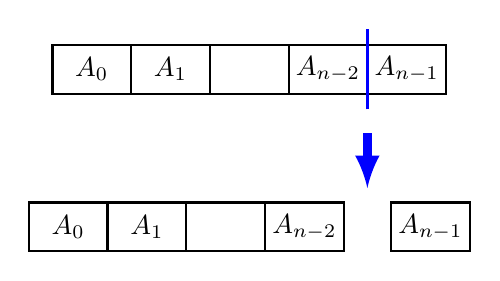
\begin{tikzpicture}[scale=1.0, auto,swap]
    
     \foreach \i/\name in { 0/A_0,1/A_1,2/\hdots,3/A_{n-2},4/A_{n-1} } {
         \draw[  black, thick ] (\i,0) rectangle (\i+1, 0.618);
         \node at (\i+0.5, 0.618/2) {$\name$};
    }
 
   \draw[very thick, blue] (4,-0.2) -- (4, 0.618+0.2);
   \draw[ -latex, blue, line width=3pt ] (4, -0.5) -- (4, -1.2 ); 


     \foreach \i/\name in { 0/A_0,1/A_1,2/\hdots,  3/A_{n-2}} {
         \draw[  black, thick ] (\i-0.3,0-2) rectangle (\i+1-0.3, 0.618-2);
         \node at (\i+0.5-0.3, 0.618/2-2) {$\name$};
     }
 
      \foreach \i/\name in { 4/A_{n-1} } {
         \draw[  black, thick ] (\i+0.3,0-2) rectangle (\i+1+0.3, 0.618-2);
         \node at (\i+0.5+0.3, 0.618/2-2) {$\name$};
    }
\end{tikzpicture}
	\caption{\fangsong 依据元素下标将数组$A[0..n-1]$分解成小的数组$A[0..n-2]$和最后一个元素$A[n-1]$。}	
	\label{An}
\end{figure}

    在将原给定实例分解成子实例之后,我们假定子实例已被求解,下一步需要思考如何将子实例的解“组合”成原始给定实例的解。这里对子实例的求解就是“分而治之”里的“治”(Conquer),可以通过递归调用来完成。
    
    对数组来说,所谓子实例的解就是已经排好序的小的数组$A[0..n-2]$。要想完成对整个数组$A[0..n-1]$的排序,我们只需将$A[n-1]$和小数组$A[0..n-2]$中的元素逐个比较,然后将$A[n-1]$插入到合适的位置即可。
    
 {\bf 算法设计与描述:} 
 	采用上述问题分解方案的算法称为“\uwave{插入排序}”(Insertion Sort),用伪代码描述如下:
   
\begin{algorithm}[H]
\caption{{\sc InsertionSort} algorithm}\label{InsertionSortAlgo} 
{\bf function} {\sc InsertionSort}($A$, $n$) 
\begin{algorithmic}[1]	
%\REQUIRE{$n>0$}
\IF{$n==1$}
	\RETURN{;}
\ELSE	
	\STATE{{\sc InsertionSort}($A$, $n-1$)}; 
	\STATE{$key = A[n-1]$;}
	\STATE $i = n - 1;$
	\WHILE{$i \geq 0$ and $A[i] > key $}
		\STATE $A[i+1] = A[i];$ 
		\STATE $i--;$
	\ENDWHILE
	\STATE $A[i+1] = key;$
\ENDIF
\end{algorithmic}
\end{algorithm}
	

\begin{figure}[H]\centering
    
\begin{tikzpicture}[scale=1., auto,swap]
 
%level 1
  \foreach \i/\name in { 2/4,3/3,4/2, 5/1 } {
         \draw[  fill=white, thick ] (\i*0.5,0) rectangle (\i*0.5+0.5, 0.5);
         \node at (\i*0.5+0.25, 0.5/2) {$\name$};
 }
%%\pause
 
%level 2
	\def\f{0.25};
   \foreach \i/\name in { 1/4,2/3,3/2 } {
         \draw[  fill=white, thick ] (\i*0.5-1 -\f,0-1) rectangle (\i*0.5-1+0.5-\f, 0.5-1);
         \node at (\i*0.5+0.25-1-\f, 0.5/2-1) {$\name$};
 }
 
    \foreach \i/\name in { 6/1 } {
         \draw[  fill=white, thick ] (\i*0.5+1-\f,0-1) rectangle (\i*0.5+1+0.5-\f, 0.5-1);
         \node at (\i*0.5+0.25+1-\f, 0.5/2-1) {$\name$};
 }
 
 % line 1-2 
 \foreach \source/\dest in {{( 4*0.5 , 0)/( 2*0.5 - 1, -0.5)}, {( 4*0.5 , 0)/( 6*0.5 + 1, -0.5)}} 
 	\path[draw=red, ->, thick]  \source  --  \dest;

 \node[red, ultra thick] at (-3, -1.5) {\fangsong 实例的分解}; 
 
  
%%\pause  
  %level 3
     \foreach \i/\name in { 0/4,1/3 } {
         \draw[  fill=white, thick ] (\i*0.5-1-0.5,0-2) rectangle (\i*0.5-1+0.5-0.5, 0.5-2);
         \node at (\i*0.5+0.25-1-0.5, 0.5/2-2) {$\name$};
 }
 
      \foreach \i/\name in { 3/2 } {
         \draw[  fill=white, thick ] (\i*0.5-1+0.5-\f,0-2) rectangle (\i*0.5-1+0.5+0.5-\f, 0.5-2);
         \node at (\i*0.5+0.25-1+0.5-\f, 0.5/2-2) {$\name$};
 }
 

%line 2-3
  \foreach \source/\dest in {{( 2*0.5 - 1, -1)/( 1*0.5 - 1 -0.5, -1.5)}, {( 2*0.5 - 1, -1)/( 3*0.5 - 1 +0.5, -1.5)}%,{( 6*0.5 + 1, -1)/( 5*0.5 + 1 - 0.5, -1.5)},{( 6*0.5 + 1, -1)/( 7*0.5 + 1 + 0.5, -1.5)}
  } 
 	\path[draw=red, ->, thick]  \source  --  \dest;
  
  
%%\pause
 %level 4
      \foreach \i/\name in { 0/4 } {
         \draw[  fill=white, thick ] (\i*0.5-1-0.5 -0.25,0-3) rectangle (\i*0.5-1+0.5-0.5 -0.25, 0.5-3);
         \node at (\i*0.5+0.25-1-0.5 -0.25, 0.5/2-3) {$\name$};
 }
 
       \foreach \i/\name in { 1/3 } {
         \draw[  fill=white, thick ] (\i*0.5-1-0.5 +0.25,0-3) rectangle (\i*0.5-1+0.5-0.5 +0.25, 0.5-3);
         \node at (\i*0.5+0.25-1-0.5 + 0.25, 0.5/2-3) {$\name$};
 }
 
  
 % line 3-4
    \foreach \source/\dest in {{( 1*0.5 - 1 -0.5, -2)/( 1*0.5 - 1 -0.5 - 0.5, -2.5)}, {( 1*0.5 - 1 -0.5, -2)/( 1*0.5 - 1 -0.5 + 0.5, -2.5)}%, {( 3*0.5 - 1 +0.5, -2)/( 3*0.5 - 1 +0.5 + 0.5, -2.5)},{( 3*0.5 - 1 +0.5, -2)/( 3*0.5 - 1 +0.5 - 0.5, -2.5)}, {( 5*0.5 + 1 - 0.5, -2)/( 5*0.5 + 1 - 0.5 + 0.5, -2.5)},{( 5*0.5 + 1 - 0.5, -2)/( 5*0.5 + 1 - 0.5 - 0.5, -2.5)}, {( 7*0.5 + 1 + 0.5, -2)/( 7*0.5 + 1 + 0.5 + 0.5, -2.5)},{( 7*0.5 + 1 + 0.5, -2)/( 7*0.5 + 1 + 0.5 - 0.5, -2.5)}
    } 
 	\path[draw=red, ->, thick]  \source  --  \dest;
	
	
%%\pause
%level -3
	\def\f{0.25}
     \foreach \i/\name in { 0/3,1/4 } {
         \draw[  fill=blue!20, thick ] (\i*0.5-1-0.5,0-4) rectangle (\i*0.5-1+0.5-0.5, 0.5-4);
         \node at (\i*0.5+0.25-1-0.5, 0.5/2-4) {$\name$};
 }
 
 
 
% line  4 to -3
	\def\d{1.5}
	\def\e{0.5}
    \foreach \source/\dest in {{( 1*0.5 - 1 -0.5, -2 - \d)/( 1*0.5 - 1 -0.5 - 0.5, -2.5-\e)},{( 1*0.5 - 1 -0.5, -2- \d)/( 1*0.5 - 1 -0.5 + 0.5, -2.5- \e)}} 
 	\path[draw=blue, ->, thick]  \dest  --  \source;

 \node[blue, ultra thick] at (-3, -4.5) {\fangsong 解的组合}; 

%%\pause
      \foreach \i/\name in { 3/2 } {
         \draw[  fill=blue!20, thick ] (\i*0.5-1+0.5-\f,0-4) rectangle (\i*0.5-1+0.5+0.5-\f, 0.5-4);
         \node at (\i*0.5+0.25-1+0.5-\f, 0.5/2-4) {$\name$};
 }


%%\pause
%level -2
	\def\f{0.25}
   \foreach \i/\name in { 1/2,2/3,3/4 } {
         \draw[  fill=blue!20, thick ] (\i*0.5-1 - \f,0-5) rectangle (\i*0.5-1+0.5 - \f, 0.5-5);
         \node at (\i*0.5+0.25-1 - \f, 0.5/2-5) {$\name$};
 }
 


%line -3 to -2
	\def\d{3.5}
	\def\e{2.5}
 
  \foreach \source/\dest in {{( 2*0.5 - 1, -1 - \d)/( 1*0.5 - 1 -0.5, -1.5 - \e)}, {( 2*0.5 - 1, -1 - \d)/( 3*0.5 - 1 +0.5, -1.5 - \e)}} 
 	\path[draw=blue, ->, thick]  \dest  --  \source;

%%\pause
  	\def\f{0.25}
    \foreach \i/\name in { 6/1} {
         \draw[  fill=blue!20, thick ] (\i*0.5+1-\f,0-5) rectangle (\i*0.5+1+0.5-\f, 0.5-5);
         \node at (\i*0.5+0.25+1-\f, 0.5/2-5) {$\name$};
 }

%%\pause
%level -1
  \foreach \i/\name in { 2/1,3/2,4/3, 5/4} {
         \draw[  fill=blue!20, thick ] (\i*0.5,0-6) rectangle (\i*0.5+0.5, 0.5-6);
         \node at (\i*0.5+0.25, 0.5/2-6) {$\name$};
 }
 % line -2 to -1
  	\def\d{5.5}
	\def\e{4.5} 
 \foreach \source/\dest in {{( 4*0.5 , 0 - \d)/( 2*0.5 - 1, -0.5 - \e)}, {( 4*0.5 , 0 - \d)/( 6*0.5 + 1, -0.5 - \e)}} 
 	\path[draw=blue, ->, thick]    \dest -- \source;

  
\end{tikzpicture}
\caption{\fangsong {\sc InsertionSort}算法对$n=4$的一个数组的排序过程。}
\label{InsertionSortExample}\end{figure}

%
%\begin{figure}[H]\centering\centering
%\begin{tikzpicture}[scale=0.9, auto,swap]
%  
%  	\def\d{0.5};
%	
% 	\def\dy{3};
%	\def\dx{-3};
%    \foreach \i/\num/\name in { 0/8/s8,1/7/s7,2/6/s6,3/5/s5,4/4/s4,5/3/s3, 6/2/s2, 7/1/s1} {
%         \draw[  thick ] (\i*\d + \dx,0+\dy) rectangle (\i*\d+\d + \dx, \d + \dy);
%         \node (\name) at (\i*\d+\d/2 + \dx, \d/2 + \dy) {$\num$};
%    }
%
%
% 	\draw[-,blue,thick] (s8.north) to[out=30,in=180-30] (s7.north);
%
%
% 	\def\dy{1};
%	\def\dx{-3};
%    \foreach \i/\num/\name in { 0/7/s7,1/8/s8,2/6/s6,3/5/s5,4/4/s4,5/3/s3, 6/2/s2, 7/1/s1} {
%         \draw[  thick ] (\i*\d + \dx,0+\dy) rectangle (\i*\d+\d + \dx, \d + \dy);
%         \node (\name) at (\i*\d+\d/2 + \dx, \d/2 + \dy) {$\num$};
%    }
%    
%    
%
% 	\draw[-,blue,thick] (s8.north) to[out=30,in=180-30] (s7.north);
% 	\draw[-,blue,thick] (s8.north) to[out=30,in=180-30] (s6.north);
%	
% 	\draw[-,blue,thick] (s7.north) to[out=35,in=180-35] (s6.north);
%
%
%	\node at (-3 + 4*\d, 0) {$\vdots$};
%
% 	\def\dy{-2.5};
%	\def\dx{-3};
%    \foreach \i/\num/\name in { 0/1/s1,1/2/s2,2/3/s3,3/4/s4,4/5/s5,5/6/s6, 6/7/s7, 7/8/s8} {
%         \draw[  thick ] (\i*\d + \dx,0+\dy) rectangle (\i*\d+\d + \dx, \d + \dy);
%         \node (\name) at (\i*\d+\d/2 + \dx, \d/2 + \dy) {$\num$};
%    }
%    
%    \node at (-3 + 4*\d, -3) {{\sc InsertSort}: 28 ops};
%
%
% 	\draw[-,blue,thick] (s8.north) to[out=180-30,in=30] (s7.north);
% 	\draw[-,blue,thick] (s8.north) to[out=180-35,in=35] (s6.north);
% 	\draw[-,blue,thick] (s8.north) to[out=180-40,in=40] (s5.north);
% 	\draw[-,blue,thick] (s8.north) to[out=180-45,in=45] (s4.north);
% 	\draw[-,blue,thick] (s8.north) to[out=180-50,in=50] (s3.north);
% 	\draw[-,blue,thick] (s8.north) to[out=180-55,in=55] (s2.north);
% 	\draw[-,blue,thick] (s8.north) to[out=180-60,in=60] (s1.north);
%	
%	\draw[-,blue,thick] (s7.north) to[out=180-30,in=30] (s6.north);
% 	\draw[-,blue,thick] (s7.north) to[out=180-35,in=35] (s5.north);
% 	\draw[-,blue,thick] (s7.north) to[out=180-40,in=40] (s4.north);
% 	\draw[-,blue,thick] (s7.north) to[out=180-45,in=45] (s3.north);
% 	\draw[-,blue,thick] (s7.north) to[out=180-50,in=50] (s2.north);
% 	\draw[-,blue,thick] (s7.north) to[out=180-55,in=55] (s1.north);
%
%	\draw[-,blue,thick] (s6.north) to[out=180-30,in=30] (s5.north);
% 	\draw[-,blue,thick] (s6.north) to[out=180-35,in=35] (s4.north);
% 	\draw[-,blue,thick] (s6.north) to[out=180-40,in=40] (s3.north);
% 	\draw[-,blue,thick] (s6.north) to[out=180-45,in=45] (s1.north);
% 	\draw[-,blue,thick] (s6.north) to[out=180-50,in=50] (s1.north);
%
%	\draw[-,blue,thick] (s5.north) to[out=180-30,in=30] (s4.north);
% 	\draw[-,blue,thick] (s5.north) to[out=180-35,in=35] (s3.north);
% 	\draw[-,blue,thick] (s5.north) to[out=180-40,in=40] (s2.north);
% 	\draw[-,blue,thick] (s5.north) to[out=180-45,in=45] (s1.north);
%
%	\draw[-,blue,thick] (s4.north) to[out=180-30,in=30] (s3.north);
% 	\draw[-,blue,thick] (s4.north) to[out=180-35,in=35] (s2.north);
% 	\draw[-,blue,thick] (s4.north) to[out=180-40,in=40] (s1.north);
%
%	\draw[-,blue,thick] (s3.north) to[out=180-30,in=30] (s2.north);
% 	\draw[-,blue,thick] (s3.north) to[out=180-35,in=35] (s1.north);
%
%	\draw[-,blue,thick] (s2.north) to[out=180-30,in=30] (s1.north);
%
%
%\end{tikzpicture}
%
%\end{figure}
%
	

{\bf 插入排序算法的时间复杂度分析:}
图\ref{InsertionSortExample}展示{\sc InsertionSort}算法对$n=4$的一个数组的排序过程。由于初始数组是逆序排列的,因此在“组合”解时,共需要执行6次比较操作和赋值操作。我们用$T(n)$表示{\sc InsertionSort}算法的时间复杂度,得到如下的递归关系:
\[
	T(n) = \begin{cases} 
		1 & \text{ 如果} n = 1 \nonumber \\ 
	 T(n-1) + O(n)  & \text{ 否则}  \nonumber 
	 	\end{cases}
\]
其中$O(n)$表示“组合”解的时间(在最坏情况下,第$8-11$行的{\tt while}循环需要执行$O(n)$轮)。

为获得$T(n)$上界的显式表达式,我们将上述递归表达式展开,得到如下结果:
\begin{eqnarray}
T(n) &\leq& T(n-1) + c n \nonumber \\ 
       &\leq& T(n-2) + c (n-1) + c n \nonumber \\
       & & \cdots \cdots \nonumber \\ 
       &\leq& c + \cdots + c (n-1) + c n \nonumber \\
       &=& O(n^{2}) \nonumber 
\end{eqnarray}
此处的$c$是为了分析方便而引入的一个常数。

{\sc InsertionSort}算法时间复杂度较高,对于大数组来说运行速度很慢,故而不实用。算法低效的原因是:在运行过程中,\uwave{问题规模是线性下降的},即每次递归操作都是将规模为$n$的问题分解成一个规模为$n-1$的子问题。



\subsubsection*{第二种分解方案及相应的{\sc MergeSort}算法}

{\bf 基本思想:}
下面我们来看另外一种问题分解方法,能够使得\uwave{问题规模成指数下降}。如图\ref{An2Halves}所示,我们可以将大的数组$A[0..n-1]$按下标切成规模相同的两半,即$A[0..\lceil\frac{n}{2}\rceil-1]$和$A[\lceil\frac{n}{2}\rceil..n-1]$;每一半依然是数组,形式相同,但是规模变小,因此是原给定实例的子实例。迭代执行分解操作,即可使得问题规模成指数形式下降。

 
\begin{figure}[H]\centering\centering
    
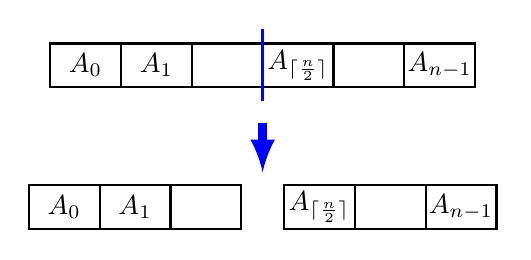
\begin{tikzpicture}[scale=0.9, auto,swap]
  
    \foreach \i/\name in { 0/A_0,1/A_1,2/\hdots,3/A_{\lceil\frac{n}{2}\rceil},4/\hdots,5/A_{n-1} } {
         \draw[  black, thick ] (\i,0) rectangle (\i+1, 0.618);
         \node at (\i+0.5, 0.618/2) {$\name$};
 }
 
   \draw[very thick, blue] (3,-0.2) -- (3,0.618+0.2);
   \draw[ -latex, blue, line width=3pt ] (3, -0.5) -- (3, -1.2 ); 


     \foreach \i/\name in { 0/A_0,1/A_1,2/\hdots } {
         \draw[  black, thick ] (\i-0.3,0-2) rectangle (\i+1-0.3, 0.618-2);
         \node at (\i+0.5-0.3, 0.618/2-2) {$\name$};
 }
 
      \foreach \i/\name in { 3/A_{\lceil\frac{n}{2}\rceil},4/\hdots,5/A_{n-1} } {
         \draw[  black, thick ] (\i+0.3,0-2) rectangle (\i+1+0.3, 0.618-2);
         \node at (\i+0.5+0.3, 0.618/2-2) {$\name$};
 }
\end{tikzpicture}
	\caption{\fangsong 依据元素下标将数组$A[0..n-1]$分解成两个小的数组:左一半$A[0..\lceil\frac{n}{2}\rceil-1]$和右一半$A[\lceil\frac{n}{2}\rceil..n-1]$。}	
	\label{An2Halves}
\end{figure}


在使用递归调用将小的数组排好序之后,我们只需依据这两个已排好序的小的数组,“归并”(Merge)出整个数组。这里的归并包括两层意思:合并、以及排序。


{\bf 算法设计与描述:} 采用这种实例分解方式的排序算法称作“归并排序”(Merge sort)\cite{Neumann1945MergeSort},伪代码描述如下:

\begin{algorithm}[H]
\caption{{\sc MergeSort} algorithm: Sort elements in $A[l..r]$} \label{MergeSortAlgo} 
{\bf function} {\sc MergeSort}$( A, l, r )$
\begin{algorithmic}[1] 
\IF{$ l < r$ }
	\STATE $m = \lceil( l + r )/ 2\rceil; $ //$m$ denotes the middle point
	\STATE {\sc MergeSort}($A, l, m$ ); 
	\STATE {\sc MergeSort}($A,m+1, r$); 
	\STATE {\sc Merge}($A, l, m, r$); //Merge the sorted arrays 
\ENDIF
\end{algorithmic}
\end{algorithm}

上述代码是对数组$A$中下标$l$到$r$之间的元素进行排序;我们执行{\sc MergeSort}$(A, 0, n-1)$即可完成对整个数组的排序。算法中的{\sc Merge}函数完成归并操作,可以这样来直观理解:整体数组的最小元素要么是小数组$A[l..m]$的最小元素(由于小数组$A[l..m]$已排好序,最小元素存放于$A[l]$中),要么是小数组$A[m+1..r]$的最小元素(由于小数组$A[m+1..r]$已排好序,最小元素存放于$A[m+1]$中),因此只需将这两个最小元素做比较即可。如此循环$n$次,即可完成整个数组$A[0..n-1]$的排序。归并过程见图\ref{merge}),伪代码表示如下:


\begin{algorithm}[H]
\caption{Merge presorted $A[l..m]$ (denoted as $L$) and $A[m+1..r]$  (denoted as $R$)} \label{MergeAlgo} 
{\bf function} {\sc Merge}$(A, l, m, r )$
\begin{algorithmic}[1]
\STATE $i=0;$ $j=0;$
\FOR{$k = l $ to $r$}
	\IF{$L[i] > R[j]$}
		\STATE $A[k] = R[j];$
		\STATE $j++;$
	\ELSE
		\STATE $A[k] = L[i];$
		\STATE $i++;$
	\ENDIF
\ENDFOR
\end{algorithmic}
\end{algorithm}


\begin{figure}[H]\centering 
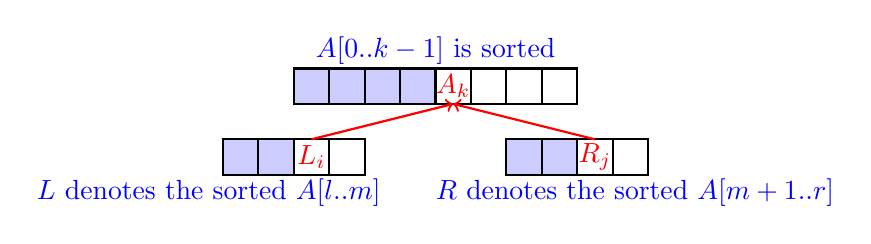
\begin{tikzpicture}[scale=0.9, auto,swap]
 
  \foreach \i/\name in { 0/,1/,2/,3/ } {
         \draw[  fill=blue!20, thick ] (\i*0.5,0) rectangle (\i*0.5+0.5, 0.5);
         \node at (\i*0.5+0.25, 0.5/2) {$\name$};
 }
 
 
  \foreach \i/\name in { 4/A_k, 5/, 6/, 7/ } {
         \draw[   thick ] (\i*0.5,0) rectangle (\i*0.5+0.5, 0.5);
         \node[red] at (\i*0.5+0.25, 0.5/2) {$\name$};
 }
 

 %level 2
     \foreach \i/\name in { 0/,1/,2/L_i,3/ } {
         \draw[  fill=blue!20, thick ] (\i*0.5-1,0-1) rectangle (\i*0.5-1+0.5, 0.5-1);
         \node[red] at (\i*0.5+0.25-1, 0.5/2-1) {$\name$};
 }

  
   \foreach \i/\name in { 2/L_i,3/ } {
         \draw[  fill=white, thick ] (\i*0.5-1,0-1) rectangle (\i*0.5-1+0.5, 0.5-1);
         \node[red] at (\i*0.5+0.25-1, 0.5/2-1) {$\name$};
 }
 
    \foreach \i/\name in { 4/, 5/, 6/R_j, 7/} {
         \draw[  fill=blue!20, thick ] (\i*0.5+1,0-1) rectangle (\i*0.5+1+0.5, 0.5-1);
         \node[red] at (\i*0.5+0.25+1, 0.5/2-1) {$\name$};
 }

    \foreach \i/\name in {  6/R_j, 7/} {
         \draw[  fill=white, thick ] (\i*0.5+1,0-1) rectangle (\i*0.5+1+0.5, 0.5-1);
         \node[red] at (\i*0.5+0.25+1, 0.5/2-1) {$\name$};
 }
    

 % lines 
 \foreach \source/\dest in {{( 4*0.5 + 0.25, 0)/( 2*0.5 - 1 + 0.25, -0.5)}, {( 4*0.5 + 0.25, 0)/( 6*0.5 + 1 + 0.25, -0.5)}} 
 	\path[draw=red, <-, thick]  \source  --  \dest;
 
\node[blue] at (2, 0.5/2-1.5) {$L$ denotes the sorted $A[l..m]$\qquad $R$ denotes the sorted $A[m+1..r]$};
\node[blue] at (2, 0.75) { $A[0..k-1]$ is sorted};
    
\end{tikzpicture}
\caption{\fangsong 归并过程:将已排好序的两个小数组$A[l..m]$和$A[m+1..r]$合并,并整理成有序数组$A[0..n-1]$。}
\label{MergeExample}
\end{figure}





\begin{figure}[H]\centering
    
\begin{tikzpicture}[scale=1., auto,swap]
 
%level 1
  \foreach \i/\name in { 0/8,1/7,2/6,3/5,4/4, 5/3, 6/2, 7/1 } {
         \draw[  fill=white, thick ] (\i*0.5,0) rectangle (\i*0.5+0.5, 0.5);
         \node at (\i*0.5+0.25, 0.5/2) {$\name$};
 }
%\pause
 
%level 2
   \foreach \i/\name in { 0/8,1/7,2/6,3/5 } {
         \draw[  fill=white, thick ] (\i*0.5-1,0-1) rectangle (\i*0.5-1+0.5, 0.5-1);
         \node at (\i*0.5+0.25-1, 0.5/2-1) {$\name$};
 }
 
    \foreach \i/\name in { 4/4, 5/3, 6/2, 7/1 } {
         \draw[  fill=white, thick ] (\i*0.5+1,0-1) rectangle (\i*0.5+1+0.5, 0.5-1);
         \node at (\i*0.5+0.25+1, 0.5/2-1) {$\name$};
 }
 
 % line 1-2 
 \foreach \source/\dest in {{( 4*0.5 , 0)/( 2*0.5 - 1, -0.5)}, {( 4*0.5 , 0)/( 6*0.5 + 1, -0.5)}} 
 	\path[draw=red, ->, thick]  \source  --  \dest;

 \node[red, ultra thick] at (-3, -1.5) {\fangsong 实例的分解}; 
 
  
%\pause  
  %level 3
     \foreach \i/\name in { 0/8,1/7 } {
         \draw[  fill=white, thick ] (\i*0.5-1-0.5,0-2) rectangle (\i*0.5-1+0.5-0.5, 0.5-2);
         \node at (\i*0.5+0.25-1-0.5, 0.5/2-2) {$\name$};
 }
 
      \foreach \i/\name in { 2/6,3/5 } {
         \draw[  fill=white, thick ] (\i*0.5-1+0.5,0-2) rectangle (\i*0.5-1+0.5+0.5, 0.5-2);
         \node at (\i*0.5+0.25-1+0.5, 0.5/2-2) {$\name$};
 }
 
     \foreach \i/\name in { 4/4, 5/3 } {
         \draw[  fill=white, thick ] (\i*0.5+1-0.5,0-2) rectangle (\i*0.5+1+0.5-0.5, 0.5-2);
         \node at (\i*0.5+0.25+1-0.5, 0.5/2-2) {$\name$};
 }
 
      \foreach \i/\name in { 6/2, 7/1 } {
         \draw[  fill=white, thick ] (\i*0.5+1+0.5,0-2) rectangle (\i*0.5+1+0.5+0.5, 0.5-2);
         \node at (\i*0.5+0.25+1+0.5, 0.5/2-2) {$\name$};
 }
%line 2-3
  \foreach \source/\dest in {{( 2*0.5 - 1, -1)/( 1*0.5 - 1 -0.5, -1.5)}, {( 2*0.5 - 1, -1)/( 3*0.5 - 1 +0.5, -1.5)},{( 6*0.5 + 1, -1)/( 5*0.5 + 1 - 0.5, -1.5)},{( 6*0.5 + 1, -1)/( 7*0.5 + 1 + 0.5, -1.5)}} 
 	\path[draw=red, ->, thick]  \source  --  \dest;
  
%\pause
 %level 4
      \foreach \i/\name in { 0/8 } {
         \draw[  fill=white, thick ] (\i*0.5-1-0.5 -0.25,0-3) rectangle (\i*0.5-1+0.5-0.5 -0.25, 0.5-3);
         \node at (\i*0.5+0.25-1-0.5 -0.25, 0.5/2-3) {$\name$};
 }
 
       \foreach \i/\name in { 1/7 } {
         \draw[  fill=white, thick ] (\i*0.5-1-0.5 +0.25,0-3) rectangle (\i*0.5-1+0.5-0.5 +0.25, 0.5-3);
         \node at (\i*0.5+0.25-1-0.5 + 0.25, 0.5/2-3) {$\name$};
 }
 
       \foreach \i/\name in { 2/6 } {
         \draw[  fill=white, thick ] (\i*0.5 - 1 + 0.5 - 0.25,0-3) rectangle (\i*0.5 - 1 + 0.5 + 0.5 - 0.25, 0.5-3);
         \node at (\i*0.5+0.25-1 + 0.5 - 0.25, 0.5/2-3) {$\name$};
 }
 
        \foreach \i/\name in { 3/5 } {
         \draw[  fill=white, thick ] (\i*0.5 - 1 + 0.5 + 0.25,0-3) rectangle (\i*0.5 - 1 + 0.5 + 0.5 + 0.25, 0.5-3);
         \node at (\i*0.5+0.25-1 + 0.5 + 0.25, 0.5/2-3) {$\name$};
 }


     \foreach \i/\name in { 4/4 } {
         \draw[  fill=white, thick ] (\i*0.5+1-0.5 - 0.25 ,0-3) rectangle (\i*0.5+1+0.5-0.5 - 0.25, 0.5-3);
         \node at (\i*0.5+0.25+1-0.5 -0.25, 0.5/2-3) {$\name$};
 }
 
      \foreach \i/\name in {  5/3 } {
         \draw[  fill=white, thick ] (\i*0.5+1-0.5 + 0.25 ,0-3) rectangle (\i*0.5+1+0.5-0.5+ 0.25, 0.5-3);
         \node at (\i*0.5+0.25+1-0.5+ 0.25, 0.5/2-3) {$\name$};
 }
 
      \foreach \i/\name in { 6/2 } {
         \draw[  fill=white, thick ] (\i*0.5+1+0.5 - 0.25,0-3) rectangle (\i*0.5+1+0.5+0.5 - 0.25, 0.5-3);
         \node at (\i*0.5+0.25+1+0.5 - 0.25, 0.5/2-3) {$\name$};
 }
 
      \foreach \i/\name in { 7/1 } {
         \draw[  fill=white, thick ] (\i*0.5+1+0.5 + 0.25,0-3) rectangle (\i*0.5+1+0.5+0.5 + 0.25, 0.5-3);
         \node at (\i*0.5+0.25+1+0.5 + 0.25, 0.5/2-3) {$\name$};
 }
 
 % line 3-4
    \foreach \source/\dest in {{( 1*0.5 - 1 -0.5, -2)/( 1*0.5 - 1 -0.5 - 0.5, -2.5)}, {( 1*0.5 - 1 -0.5, -2)/( 1*0.5 - 1 -0.5 + 0.5, -2.5)}, {( 3*0.5 - 1 +0.5, -2)/( 3*0.5 - 1 +0.5 + 0.5, -2.5)},{( 3*0.5 - 1 +0.5, -2)/( 3*0.5 - 1 +0.5 - 0.5, -2.5)}, {( 5*0.5 + 1 - 0.5, -2)/( 5*0.5 + 1 - 0.5 + 0.5, -2.5)},{( 5*0.5 + 1 - 0.5, -2)/( 5*0.5 + 1 - 0.5 - 0.5, -2.5)}, {( 7*0.5 + 1 + 0.5, -2)/( 7*0.5 + 1 + 0.5 + 0.5, -2.5)},{( 7*0.5 + 1 + 0.5, -2)/( 7*0.5 + 1 + 0.5 - 0.5, -2.5)}} 
 	\path[draw=red, ->, thick]  \source  --  \dest;
	
%\pause
%level -3
     \foreach \i/\name in { 0/7,1/8 } {
         \draw[  fill=blue!20, thick ] (\i*0.5-1-0.5,0-4) rectangle (\i*0.5-1+0.5-0.5, 0.5-4);
         \node at (\i*0.5+0.25-1-0.5, 0.5/2-4) {$\name$};
 }
 
      \foreach \i/\name in { 2/5,3/6 } {
         \draw[  fill=blue!20, thick ] (\i*0.5-1+0.5,0-4) rectangle (\i*0.5-1+0.5+0.5, 0.5-4);
         \node at (\i*0.5+0.25-1+0.5, 0.5/2-4) {$\name$};
 }
 
     \foreach \i/\name in { 4/3, 5/4 } {
         \draw[  fill=blue!20, thick ] (\i*0.5+1-0.5,0-4) rectangle (\i*0.5+1+0.5-0.5, 0.5-4);
         \node at (\i*0.5+0.25+1-0.5, 0.5/2-4) {$\name$};
 }
 
      \foreach \i/\name in { 6/1, 7/2 } {
         \draw[  fill=blue!20, thick ] (\i*0.5+1+0.5,0-4) rectangle (\i*0.5+1+0.5+0.5, 0.5-4);
         \node at (\i*0.5+0.25+1+0.5, 0.5/2-4) {$\name$};
 }
 
% line  4 to -3
	\def\d{1.5}
	\def\e{0.5}
    \foreach \source/\dest in {{( 1*0.5 - 1 -0.5, -2 - \d)/( 1*0.5 - 1 -0.5 - 0.5, -2.5-\e)}, {( 1*0.5 - 1 -0.5, -2 - \d)/( 1*0.5 - 1 -0.5 + 0.5, -2.5 - \e)}, {( 3*0.5 - 1 +0.5, -2 - \d)/( 3*0.5 - 1 +0.5 + 0.5, -2.5 - \e)},{( 3*0.5 - 1 +0.5, -2 - \d)/( 3*0.5 - 1 +0.5 - 0.5, -2.5 - \e)}, {( 5*0.5 + 1 - 0.5, -2 - \d)/( 5*0.5 + 1 - 0.5 + 0.5, -2.5 - \e)},{( 5*0.5 + 1 - 0.5, -2 - \d)/( 5*0.5 + 1 - 0.5 - 0.5, -2.5 - \e)}, {( 7*0.5 + 1 + 0.5, -2 - \d)/( 7*0.5 + 1 + 0.5 + 0.5, -2.5 - \e)},{( 7*0.5 + 1 + 0.5, -2 - \d)/( 7*0.5 + 1 + 0.5 - 0.5, -2.5 - \e)}} 
 	\path[draw=blue, ->, thick]  \dest  --  \source;

 \node[blue, ultra thick] at (-3, -4.5) {\fangsong 组合子实例的解}; 


%\pause
%level -2
   \foreach \i/\name in { 0/5,1/6,2/7,3/8 } {
         \draw[  fill=blue!20, thick ] (\i*0.5-1,0-5) rectangle (\i*0.5-1+0.5, 0.5-5);
         \node at (\i*0.5+0.25-1, 0.5/2-5) {$\name$};
 }
 
    \foreach \i/\name in { 4/1, 5/2, 6/3, 7/4 } {
         \draw[  fill=blue!20, thick ] (\i*0.5+1,0-5) rectangle (\i*0.5+1+0.5, 0.5-5);
         \node at (\i*0.5+0.25+1, 0.5/2-5) {$\name$};
 }

%line -3 to -2
	\def\d{3.5}
	\def\e{2.5}
 
  \foreach \source/\dest in {{( 2*0.5 - 1, -1 - \d)/( 1*0.5 - 1 -0.5, -1.5 - \e)}, {( 2*0.5 - 1, -1 - \d)/( 3*0.5 - 1 +0.5, -1.5 - \e)},{( 6*0.5 + 1, -1 - \d)/( 5*0.5 + 1 - 0.5, -1.5 - \e)},{( 6*0.5 + 1, -1 - \d)/( 7*0.5 + 1 + 0.5, -1.5 - \e)}} 
 	\path[draw=blue, ->, thick]  \dest  --  \source;

%\pause
%level 1
  \foreach \i/\name in { 0/1,1/2,2/3,3/4,4/5, 5/6, 6/7, 7/8 } {
         \draw[  fill=blue!20, thick ] (\i*0.5,0-6) rectangle (\i*0.5+0.5, 0.5-6);
         \node at (\i*0.5+0.25, 0.5/2-6) {$\name$};
 }
 % line 1-2
 	\def\d{5.5}
	\def\e{4.5} 
 \foreach \source/\dest in {{( 4*0.5 , 0 - \d)/( 2*0.5 - 1, -0.5 - \e)}, {( 4*0.5 , 0 - \d)/( 6*0.5 + 1, -0.5 - \e)}} 
 	\path[draw=blue, ->, thick]    \dest -- \source;

  
\end{tikzpicture}
\caption{\fangsong {\sc MergeSort}算法对$n=8$的一个数组的运行过程。}
\label{MergeSortExample}
\end{figure}

\begin{figure}[H]\centering
    
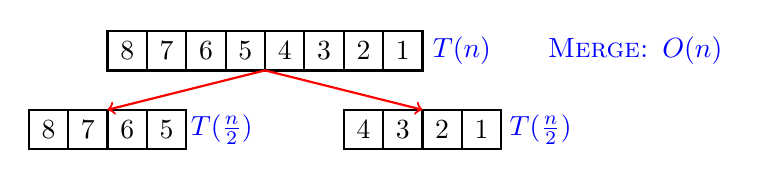
\begin{tikzpicture}[scale=1., auto,swap]
 
  \foreach \i/\name in { 0/8,1/7,2/6,3/5,4/4, 5/3, 6/2, 7/1 } {
         \draw[  fill=white, thick ] (\i*0.5,0) rectangle (\i*0.5+0.5, 0.5);
         \node at (\i*0.5+0.25, 0.5/2) {$\name$};
 }
 
 \node[blue] at (8*0.5 + 0.5, 0.5/2) {$T(n)$};
  \node[blue] at (8*0.5 + 2.7, 0.5/2) {{\sc Merge: }$O(n)$};
 \node[blue] at (4*0.5-0.55 , 0.5/2-1) {$T(\frac{n}{2})$};
 \node[blue] at (8*0.5 + 1.5, 0.5/2-1) {$T(\frac{n}{2})$};
 
 %level 2
  
   \foreach \i/\name in { 0/8,1/7,2/6,3/5 } {
         \draw[  fill=white, thick ] (\i*0.5-1,0-1) rectangle (\i*0.5-1+0.5, 0.5-1);
         \node at (\i*0.5+0.25-1, 0.5/2-1) {$\name$};
 }
 
    \foreach \i/\name in { 4/4, 5/3, 6/2, 7/1 } {
         \draw[  fill=white, thick ] (\i*0.5+1,0-1) rectangle (\i*0.5+1+0.5, 0.5-1);
         \node at (\i*0.5+0.25+1, 0.5/2-1) {$\name$};
 }
  
  
 % lines 
 \foreach \source/\dest in {{( 4*0.5 , 0)/( 2*0.5 - 1, -0.5)}, {( 4*0.5 , 0)/( 6*0.5 + 1, -0.5)}} 
 	\path[draw=red, ->, thick]  \source  --  \dest;
 
	
  
\end{tikzpicture}
\caption{\fangsong 归并排序算法的时间复杂度分析:以$n=8$的一个数组为例。}
\label{mergesortcomplexity}
\end{figure}

{\bf  归并排序算法的时间复杂度分析:} 
图\ref{MergeSortExample}展示了{\sc MergeSort}算法对$n=8$的一个数组的运行过程。我们注意到使用{\sc Merge}函数对整个数组$A[0..n-1]$进行排序时,需要执行$n$次{\tt for}循环(第2-10行),需要$O(n)$的时间。我们以$T(n)$表示对数组$A[0..n-1]$运行{\sc MergeSort}的时间。由于两个小的数组的递归调用时间为$2  T(\tfrac{n}{2})$,归并时间为$O(n)$(见图\ref{mergesortcomplexity}),从而得到如下递归表达式:
\[
	T(n) = \begin{cases} 
		1 & \text{ 如果} n = 1 \nonumber \\ 
	2 T(\tfrac{n}{2}) + O(n)  & \text{ 否则}  \nonumber 
	 	\end{cases}
\]

为获得时间复杂度的显式表达式,我们连续应用递归表达式,生成一颗递归树。如图\ref{mergesortree}所示,每一个结点表示一个实例;每一层所有实例的归并时间累加后都是$cn$,显示于右侧;树的叶子节点对应于分解到最后得到的最简单实例,累计时间为$n$。由于树的高度为$\log_2 n$,因此有:
\[
	T(n) = O(n \log n)
\]


和{\sc MergeSort}算法相比,{\sc InsertionSort}算法具有显著的优势,这种优势来源于归并时避免了一些冗余的比较和赋值操作。以图\ref{mergesortexample}中最下面一行所示的归并为例:我们只需比较左一半的最小元$5$和右一半的最小元$1$,即可知道总体的最小元为$1$;由于左一半已经排好序,因此无需再将$1$和左一半的其他元素$6, 7, 8$进行比较。反观{\sc MergeSort}算法的最后一次迭代,在通过比较确定了$1$的正确位置之后,需要执行$n$次移动元素操作,才能把$1$放入正确位置。


\begin{figure}[H]\centering
    
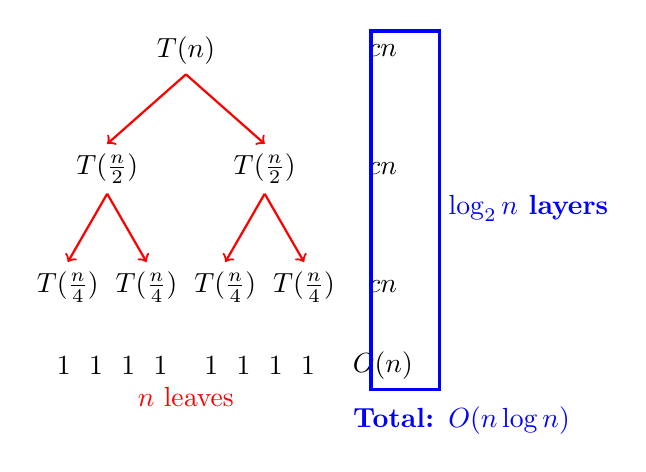
\begin{tikzpicture}[scale=1., auto,swap]
 %l1
 \node[ ] (l1) at (0,0) {$T(n)$};
 
 
 %l2
 \node[ ] (l21) at (-1,-1.5) {$T(\frac{n}{2})$};
 \node[ ] (l22) at (1,-1.5) {$T(\frac{n}{2})$};
 %l3
 \node[ ] (l31) at (-1 - 0.5,-3) {$T(\frac{n}{4})$};
 \node[ ] (l32) at (-1 + 0.5,-3) {$T(\frac{n}{4})$};
 
  \node[ ] (l33) at (1 - 0.5,-3) {$T(\frac{n}{4})$};
 \node[ ] (l34) at (1 + 0.5,-3) {$T(\frac{n}{4})$};
 
 %lines
 \path[draw,  red,->, thick] (l1.south) -- (l21.north); 
  \path[draw, red,->, thick] (l1.south) -- (l22.north);
   
 \path[draw,  red,->, thick] (l21.south) -- (l31.north); 
 \path[draw,  red,->, thick] (l21.south) -- (l32.north); 

 \path[draw,  red,->, thick] (l22.south) -- (l33.north); 
 \path[draw, red, ->, thick] (l22.south) -- (l34.north); 
      
      %cn
      \node[ ] (l1) at (2.5,0) {$\hdots cn$};  
      \node[ ] (l1) at (2.5,-1.5) {$\hdots cn$}; 
      \node[ ] (l1) at (2.5,-3) {$\hdots cn$}; 
  \node[ ] (l1) at (2.5,-4) {$\hdots O(n)$}; 
  
     \node[ ] (l1) at (0,-3.5) {$\hdots \hdots \hdots \hdots $}; 

     \node[ ] (l1) at (0,-4) {$1\ \ 1\ \ 1\ \ 1\ \ \ \ 1\ \ 1\ \ 1\ \ 1$}; 
              \node[ red ] (l1) at (0,-4.4) {$n$ leaves}; 

              
              %\pause
      %boxes
      \draw[ blue, very thick ]  (2.35, 0.25) rectangle (3.22, -4.3);
 %     \draw[ red, very thick ] (-2, -4.2) rectangle (2, -3.8);

%total      
 %        \node[ red ] (l1) at (0,-4.4) {$\tfrac{n}{2}$ leaves}; 
          \node[ blue ] (l1) at (4.35,-2) {\bf $\log_2 n$ layers}; 
	\node[blue] at (3.5, -4.7) {\bf Total: $O(n\log n)$ };

      
\end{tikzpicture}
\label{mergesorttree}
\caption{\fangsong {\sc MergeSort}算法执行过程中的递归关系树。}
\end{figure}



%\begin{figure}[H]\centering
%  \begin{minipage}{0.45\textwidth} 
%  \includegraphics[height=2.7in] {L5-insertsort-left.png}
% \end{minipage}
%  \begin{minipage}{0.45\textwidth} 
% \includegraphics[height=2.75in] {L5-mergesort-right.png}
% \end{minipage}
% \caption{\fangsong 插入排序与归并排序运行过程比较。}
% \label{InsertionSortAndMergeSort}
%\end{figure}
%



\subsection{“分而治之”算法的时间复杂度分析及Master定理}
在“分而治之”算法中,一种常见的情况是将一个规模为$n$的实例归结$a$个子实例,每个子实例规模都相同(记为$\tfrac{n}{b}$)。假如“组合”子实例解用时$O(n^d)$,则我们可以将时间复杂度$T(n)$递归表示如下:
\[
	T(n) = \begin{cases} 
		1 & \text{ 如果} n = 1 \nonumber \\ 
	a T(\tfrac{n}{b}) + O(n^d)  & \text{ 否则}  \nonumber 
	 	\end{cases}
\]

为得到$T(n)$上界的显式表达式,我们可以仿照上节所采用方式,画出递归关系树
,尝试迭代展开几次,观察总结规律,然后推导出显式的表达式。

对于子问题比较规整的情况,即每个子问题的规模都相同,$T(n)$上界的显式表达式已被总结成Master定理\cite{PapadimitriouBook},因此只需直接套用定理即可。Master定理陈述如下:

\begin{theorem}
 考虑递归表达式$T(n)=aT(\frac{n}{b}) + O(n^d)$,其中 $a > 1$, $b>1$,$d > 0$,则$T(n)$的上界可表示为:
\begin{enumerate}
 \item 当 $d < \log_b a $时, 有 $T(n)=O(n^{\log_b a })$;
 \item 当 $d = \log_b a $时, 有 $T(n)=O(n^{\log_b a } \log n )$;
 \item 当 $d > \log_b a $时, 有$T(n)=O( n^d )$。
 %Here, $\epsilon$ denotes a small, positive number. 
\end{enumerate}
\end{theorem}


	\begin{proof}
		迭代应用上述递归表达式,可得出:
		\begin{eqnarray}
		T(n) &=& a T(\tfrac{n}{b}) + O( n^{d} )\nonumber \\
		&\leq& a T(\tfrac{n}{b}) + c n^{d} \nonumber \\ 
		          &\leq& a ( a T(\tfrac{n}{b^{2}}) + c (\tfrac{n}{b})^{d} ) +   c n^{d} \nonumber\\ 
		          &\leq& \dots\dots  \nonumber\\ 
		          &\leq& c n^{d} ( 1 + \tfrac{a}{b^{d}} + (\tfrac{a}{b^{d}})^{2} + \hdots + (\tfrac{a}{b^{d}})^{\log_{b}{n}} ) \nonumber\\ 
		          &=&\begin{cases}
		          		O(n^{\log_b a }) & \text{如果 } d < \log_b a  \\ 
		          		O(n^{\log_b a } \log n ) & \text{如果 } d = \log_b a  \\ 
		          		O( n^d ) & \text{如果 } d > \log_b a  \\ 
		          \end{cases}\nonumber
   		\end{eqnarray}
	此处$c$表示一个大于0的常数。
	\end{proof}

我们在此列出直接应用Master定理的两个例子:

\begin{itemize}
 \item 从递归表达式$T(n) = 3 T(\frac{n}{2}) + O(n)$,可推出
$T(n) = O(n^{\log_2 3}) = O(n^{1.585})$。
 \item 从递归表达式$T(n) = 2 T(\frac{n}{2}) + O(n^2)$,可推出
$T(n)= O(n^2)$。
\end{itemize}

值得指出的是,Master定理仅适用于子实例规模都相等、且是原始实例规模的分数的情况,对于子实例规模不相等等特殊情况则不适用。对这些特殊情况,我们要么使用“先尝试展开几级、观察总结规律”的方法,要么采用“先猜测上界的形式、再加以证明”的方式。我们在第3章将会看到这种情况的例子。

\subsection{依据元素的值将大数组分解成小数组:{\sc QuickSort}算法}
无论是{\sc InsertionSort}还是{\sc MergeSort}算法,都是\uwave{依据元素的下标}将大数组分解成小数组,即选定一个元素,比这个元素\uwave{下标小}的元素组成一个小数组,比这个元素\uwave{下标大}的那些元素组成另一个小数组。

除了依据元素下标之外,我们还可以\uwave{依据元素的数值}将大数组分解成小数组,即选定一个元素作“\uwave{中心元}”(Pivot),比中心元\uwave{数值小}的元素组成一个小数组,比中心元\uwave{数值大}的那些元素组成另一个小数组。采用这种分解方式的排序算法称为{\sc QuickSort}算法\cite{Hoare1961},其伪代码描述如下:

\begin{algorithm}[H]
\caption{{\sc QuickSort} algorithm}\label{QuickSortAlgo} 
{\bf function} {\sc QuickSort}($A$) 
\begin{algorithmic}[1]
\STATE{Create two empty arrays $S_{-}$ and $S_{+}$;}
\STATE Choose an element $A[j]$ from $A$ \textcolor{red}{\bf uniformly at random} and use it as pivot;
\FOR{$i=0 $ to $|A|-1$}
	\IF{$A[i] < A[j]$}  
		\STATE Put $A[i]$ into $S_{-}$;
	\ELSE 
		\STATE Put $A[i]$ into $S_{+}$; 
	\ENDIF
\ENDFOR
\STATE {\sc QuickSort}$(S_{+});$
\STATE {\sc QuickSort}$(S_{-});$
\STATE Return the concatenation of $S_{-}$, $A[j]$, and $S_{+}$ as $A$; 
\end{algorithmic}
\end{algorithm}


    {\sc QuickSort}算法能够完成数组排序,这一点是显而易见的(第12行),但是时间复杂度分析却有些困难:{\sc InsertionSort}和{\sc MergeSort}算法都依据元素下标进行分解,因此子实例的大小是可以控制、在运行前可以知道的。但是{\sc QuickSort}算法中依据随机选择的中心元,所得到的子实例大小在算法运行前是并不知道的。
    
    为描述方便起见,我们称排序后的数组$A$为$\tilde{A}$,因此数组$A$的最小元是$\tilde{A}[0]$,最大元是$\tilde{A}[n-1]$,中位数是$\tilde{A}[\lceil\frac{n}{2}\rceil]$。我们在选择中心元时可能面临如下两种情况:
    \begin{enumerate}[(1)]
 \item 
{\bf 选择数组中的最大元$\tilde{A}[n-1]$/最小元$\tilde{A}[0]$作为中心元:}  这样只会生成一个子实例,规模减少了1,成线性降低。如果在每一次迭代都是如此选择的话,运行过程就与{\sc InsertionSort}算法相同,时间复杂度为:
\begin{center}
$T(n) = T(n-1) + O(n) = O(n^2)$
\end{center}

\item {\bf 选择数组中的中位数$\tilde{A}[\lceil\frac{n}{2}\rceil]$作为中心元:}  这样会生成两个子实例,每个子实例的规模都是原来的一半,成指数下降。如果在每一次迭代都是如此选择的话,运行过程就与{\sc MergeSort}算法相同,时间复杂度为:
\begin{center}
$T(n) = 2T(\tfrac{n}{2}) + O(n) = O(n \log n)$
\end{center}
\end{enumerate}

由于{\sc QuickSort}算法中是均匀随机地选择一个元素作为中心元,因此上述两种选择发生的概率都很小,都是$\tfrac{1}{n}$。大概率的情况是既不会像第一种情况那么差,也不会像第二种情况那么好,而是和第二种情况差不多。

\begin{figure}[H]\centering
    
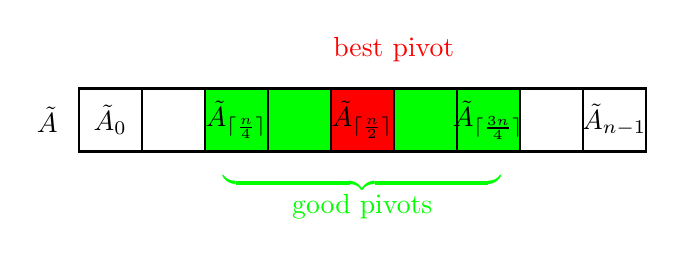
\begin{tikzpicture}[scale=1., auto,swap]
 

 \node at (-1*0.8+0.4, 0.8/2) {$\tilde{A}$};
 
  \foreach \i/\name in { 0/\tilde{A}_0,1/\hdots,2/\tilde{A}_{\frac{n}{4}},3/\hdots,4/\tilde{A}_{\lceil\frac{n}{2}\rceil},5/\hdots,6/\tilde{A}_{\frac{3n}{4}},7/\hdots,8/\tilde{A}_{n-1}}{
           \draw[  fill=white, thick ] (\i*0.8,0) rectangle (\i*0.8+0.8, 0.8);
         \node at (\i*0.8+0.4, 0.8/2) {$\name$};
 }

  \foreach \i/\name in { 2/\tilde{A}_{\lceil\frac{n}{4}\rceil},3/\hdots,4/\tilde{A}_{\lceil\frac{n}{2}\rceil},5/\hdots,6/\tilde{A}_{\lceil\frac{3n}{4}\rceil}}{
           \draw[  fill=green, thick ] (\i*0.8,0) rectangle (\i*0.8+0.8, 0.8);
         \node at (\i*0.8+0.4, 0.8/2) {$\name$};
 }
 
   \foreach \i/\name in {4/\tilde{A}_{\lceil\frac{n}{2}\rceil}}{
           \draw[  fill=red, thick ] (\i*0.8,0) rectangle (\i*0.8+0.8, 0.8);
         \node at (\i*0.8+0.4, 0.8/2) {$\name$};
 }
 \node[red] at (5*0.8, 1.3) {best pivot};
 \node[green] at (5*0.8-0.4, -0.4) {$\underbrace{\qquad\qquad\qquad\qquad\qquad}$};
 \node[green] at (5*0.8-0.4, -0.7) {good pivots};
 
\end{tikzpicture}
\caption{\fangsong {\sc QuickSort}算法中的中心元的“最优选择”和“足够好”选择。}
\label{goodpivots}
\end{figure}

详细地说,{\sc QuickSort}算法是一个随机算法,其运行过程中包含有随机行为,导致即使以同一个数组$A$作为输入,每次运行算法进行排序的执行时间也不是一个固定值,而是一个随机变量。我们将要证明\uwave{运行时间的期望值}依然是$O(n \log n)$的。这个证明过程略显复杂,我们先来看一个易于分析的“修正版”{\sc QuickSort}算法。

\subsubsection*{{\sc ModifiedQuickSort}算法:一个复杂度易于分析的版本}
 
\begin{algorithm}[H]
\caption{{\sc ModifiedQuickSort} algorithm}\label{ModifiedQuickSortAlgo} 
{\bf function} {\sc ModifiedQuickSort}($A$) 
\begin{algorithmic}[1]
\WHILE{{\tt TRUE}}
	\STATE{Create two empty arrays $S_{-}$ and $S_{+}$;}
	\STATE Choose an element $A[j]$ from $A$ \textcolor{red}{\bf uniformly at random} and use it as pivot;
	\FOR{$i=0 $ to $|A|-1$}
		\IF{$A[i] < A[j]$}  
			\STATE Put $A[i]$ into $S_{-}$;
		\ELSE 
			\STATE Put $A[i]$ into $S_{+}$; 
		\ENDIF
	\ENDFOR	
	\IF{$\|S_{+}\| \geq \frac{n}{4}$ and $\|S_{-}\| \geq \frac{n}{4}$}
		\STATE break; //A fixed proportion of elements fall both below and above the pivot; 
	\ENDIF
\ENDWHILE
\STATE {\sc ModifiedQuickSort}$(S_{+})$;
\STATE {\sc ModifiedQuickSort}$(S_{-})$;
\STATE Return the concatenation of $S_{-}$, $A[j]$, and $S_{+}$ as $A$; 
\end{algorithmic}
\end{algorithm}

和{\sc QuickSort}算法相比,{\sc ModifiedQuickSort}算法只做了一点修改:随机选择一个元素做中心元之后,先检验一下这个中心元是否“足够好”(第8-10行);如果足够好,则继续执行后续的比较和排序,否则重新选择一个元素做中心元。所谓的中心元“足够好”,是指它位于$\tilde{A}$的中间区域,即$\tilde{A}[\lceil\frac{n}{4}\rceil..\lceil\frac{3n}{4}\rceil]$。直观上看,中位数$\tilde{A}_{\lceil\frac{n}{2}\rceil}$是中心元的“最佳选择”,而$\tilde{A}$中间区域的元素是中心元的“足够好”的选择(见图\ref{goodpivots})。

	之所以说$\tilde{A}$中间区域的元素都是“足够好”的选择,是因为如下两个事实:
\begin{enumerate}[(1)]
	\item 选中$\tilde{A}$中间区域中某个元素的概率足够高:
	
	由于中间区域中共有$\frac{n}{2}$个元素,因此第3行做一次随机选择时选中中间区域某个元素的概率是$\frac{1}{2}$,进而可以推出算法中{\tt while}循环期望执行2次(一个直观的类比是掷一枚均匀硬币,等待第一次掷出正面的期望时间是2)。
	
	注意到每次{\tt while}循环里,都会将数组中的所有元素和中心元进行比较,因此递归调用之外的所有操作(即第1-14行)期望执行时间是$2n$。
	

	\item 以$\tilde{A}$中间区域中某个元素做中心元,生成子实例的规模成指数下降:中心元的最优选择是中位数$\tilde{A}_{\lceil\frac{n}{2}\rceil}$,能够产生两个规模都是$\frac{n}{2}$的子实例;选择中间区域的元素作为中心元,所生成的子实例规模会大于$\frac{n}{4}$,小于$\frac{3n}{4}$;直观上看既不会太大,也不会太小。
	
	我们用$T(n)$表示期望运行时间,可以得到如下结论:
\begin{eqnarray}
T(n) &\leq& T(\frac{n}{4})  + T(\frac{3n}{4}) + 2n \nonumber \\
       &\leq& (T(\frac{n}{16}) + T(\frac{3n}{16}) + 2\frac{n}{4} ) + (T(\frac{3n}{16}) + T(\frac{9n}{16}) + 2\frac{3n}{4}) + 2n \nonumber \\
       &=&   (T(\frac{n}{16}) + T(\frac{3n}{16})) + (T(\frac{3n}{16}) + T(\frac{9n}{16}) ) + 2n + 2n \nonumber \\ 
       &\leq& \cdots \cdots \cdots \nonumber \\
       &=& O(n \log_{\tfrac{4}{3}} n ) \nonumber 
 \end{eqnarray}

\end{enumerate}




\subsubsection*{{\sc  QuickSort}算法时间复杂度分析}
接下来我们分析{\sc  QuickSort}算法的时间复杂度。在做具体的分析之前,我们先指出关于运行时间的3点事实:
\begin{enumerate}[(1)] 
	\item 运行时间由比较次数界定:我们定义$X$为执行算法第4行中的比较操作的总次数。如果我们把所有的递归操作都展开的话,很明显算法的总运行时间由$X$确定;我们的目标就是计算$E(X)$。
	\item 任意两个元素$\tilde{A}[i]$和$\tilde{A}[j]$最多只会比较一次:如图\ref{quicksortcomparison}所示,只有当$\tilde{A}[i]$或$\tilde{A}[j]$被选做中心元时,$\tilde{A}[i]$才会和$\tilde{A}[j]$进行比较;一旦比较完成之后,$\tilde{A}[i]$和$\tilde{A}[j]$不会同时出现在$S_{-}$或者$S_{+}$中,因此不会再次进行比较)。
	
	因此我们可以定义如下的\uwave{指示变量}(Index variable):
\[
	X_{ij} = \begin{cases}
		1 & \text{ 如果元素} \tilde{A}[i]\text{和}\tilde{A}[j]\text{发生比较} \nonumber \\ 
		0 & \text{否则} \nonumber 
	\end{cases}
\]
并可以将$X$ 表示成$X = \sum\limits_{i=0}^{n-1}\sum\limits_{j=i+1}^{n-1} X_{ij}$。

\begin{figure}[H]\centering
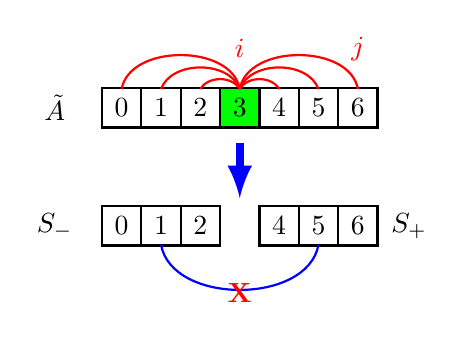
\begin{tikzpicture}[scale=1., auto,swap]
 
  \foreach \i/\name in { 0/0,1/1,2/2,3/3,4/4, 5/5, 6/6} {
         \draw[  fill=white, thick ]  (\i*0.5,0) rectangle (\i*0.5+0.5, 0.5);
         \node (U\name) at (\i*0.5+0.25, 0.5/2 ) {$\name$};
 }

 
   \foreach \i/\name in { 3/3} {
         \draw[  fill=green, thick ]  (\i*0.5,0) rectangle (\i*0.5+0.5, 0.5);
         \node (U\name) at (\i*0.5+0.25, 0.5/2 ) {$\name$};
 }
 
 %level 2
  
   \foreach \i/\name in { 0/0,1/1,2/2 } {
         \draw[  fill=white, thick ]  (\i*0.5 ,0-1.5) rectangle (\i*0.5 +0.5, 0.5-1.5);
         \node (B\name) at (\i*0.5+0.25 , 0.5/2-1.5) {$\name$};
 }
 
    \foreach \i/\name in { 4/4, 5/5, 6/6 } {
         \draw[  fill=white, thick ]   (\i*0.5  ,0-1.5) rectangle (\i*0.5 +0.5, 0.5-1.5);
         \node (B\name) at (\i*0.5+0.25 , 0.5/2-1.5) {$\name$};
 }
 %arrow
 \draw[blue, -latex, line width=3pt] (4*0.5-0.25, -0.2) -- (4*0.5-0.25, -0.9);
  %arc
  \draw[red, thick] (U3.north) to [out=60,in=180-60] (U4.north);
  \draw[red, thick] (U3.north) to [out=70,in=180-70] (U5.north);
  \draw[red, thick] (U3.north) to [out=80,in=180-80] (U6.north);	
  
    \draw[red, thick] (U3.north) to [out=180-60,in=60] (U2.north);
  \draw[red, thick] (U3.north) to [out=180-70,in=70] (U1.north);
  \draw[red, thick] (U3.north) to [out=180-80,in=80] (U0.north);	
  
    \draw[blue, thick] (B1.south) to [out=-80,in=260] (B5.south);	
    
   %no comparison 
   \node[red, thick] at (4*0.5-0.25, -2.1) {\bf X};
    \node[red, thick] at (4*0.5-0.25, 1) {$i$};
      \node[red, thick] at (7*0.5-0.25, 1) {$j$};

     \node[ thick] at (-0.6, -1.25) {$S_{-}$};
     \node[ thick] at (7*0.5 + 0.4, -1.25) {$S_{+}$};
     \node[ thick] at (-0.6, 0.25 ) {$\tilde{A}$};

\end{tikzpicture}
\caption{在{\sc QuickSort}算法执行过程中,$\tilde{A}[i]$和$\tilde{A}[j]$最多只会比较一次。}
\label{quicksortcomparison}
\end{figure}

	\item $\tilde{A}[i]$和$\tilde{A}[j]$ $(0\leq i< j\leq n-1)$发生比较的概率是$\frac{2}{j-i+1}$:对这个事实的证明我们稍后陈述。
\end{enumerate}

基于上述事实,我们立刻能够证明如下定理:
\begin{theorem}
{\sc QuickSort}算法的\uwave{期望运行时间}是
$E(X) = O(n \log n)$。
\end{theorem}
\begin{proof}
由于$X = \sum\limits_{i=0}^{n-1}\sum\limits_{j=i+1}^{n-1} X_{ij}$,我们有:

      \begin{eqnarray}
      E[ X ] & = &  E [\sum\nolimits_{i=0}^{n-1}\sum\nolimits_{j=i+1}^{n-1} X_{ij} ] \nonumber \\
              & = &   \sum\nolimits_{i=0}^{n-1}\sum\nolimits_{j=i+1}^{n-1} E[ X_{ij} ] \nonumber \\
              & = &   \sum\nolimits_{i=0}^{n-1}\sum\nolimits_{j=i+1}^{n-1} \Pr( \tilde{A}[i]  \text{和} \tilde{A}[j] \text{进行比较})  \nonumber  \\
      & = &  \sum\nolimits_{i=0}^{n-1}\sum\nolimits_{j=i+1}^{n-1}  \frac{2}{j-i+1} \nonumber \\ 
      & = & \sum\nolimits_{i=0}^{n-1} \sum\nolimits_{k=1}^{n-i-1} \frac{2}{k+1}  \nonumber \\        
      & \leq & \sum\nolimits_{i=0}^{n-1} \sum\nolimits_{k=1}^{n-1} \frac{2}{k+1} \nonumber \\
      & = & O( n \log n ) \nonumber 
      \end{eqnarray} 
 此处$k$定义为$ k=j-i$。
\end{proof}

现在我们只遗留了一个疑问:为什么在{\sc QuickSort}算法执行过程中,任意两个元素$\tilde{A}[i]$和$\tilde{A}[j]$ $(0\leq i< j\leq n-1)$发生比较的概率是$\frac{2}{j-i+1}$,而和数组的大小无关呢?我们以$i=0$, $j=2$为例,证明$\tilde{A}[0]$和$\tilde{A}[2]$比较的概率是$\frac{2}{3}$。 我们先从两个简单的情况看起:

\begin{enumerate}[(1)]
\item 数组只包含$3$个元素的情况:

如图\ref{compareij3elements}所示,当$\tilde{A}[0]$或$\tilde{A}[2]$作为中心元时,会进行$\tilde{A}[0]$和$\tilde{A}[2]$的比较,故有:
\[
\Pr( \tilde{A}[0]\text{和}\tilde{A}[2]\text{进行比较} ) = \frac{2}{3}。
\]


\begin{figure}[H]\centering  
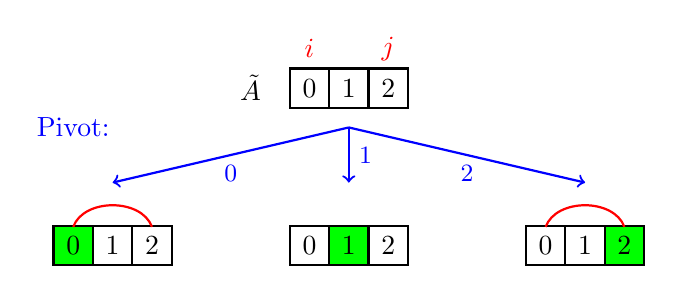
\begin{tikzpicture}[scale=1, auto,swap]
 
 %level 1
 \def\dx{0}
 \def\dy{0};

  \node[ultra thick] at ( - 0.5 + \dx, 0.25 + \dy) {$\tilde{A}$};

  \foreach \i/\name in { 0/0,1/1, 2/2} {
         \draw[  fill=white, thick ]  (\i*0.5 + \dx,0 + \dy) rectangle (\i*0.5+0.5 + \dx, 0.5 + \dy);
         \node (U\name) at (\i*0.5+0.25+ \dx, 0.5/2 + \dy) {$\name$};
 }
 
 \foreach \i/\name in { 0/0} {
         \node[ultra thick, red] at (\i*0.5+0.25+ \dx, 0.5/2 + \dy + 0.5) {$i$};
 }

 \foreach \i/\name in { 2/2} {
         \node[ultra thick, red] at (\i*0.5+0.25+ \dx, 0.5/2 + \dy + 0.5) {$j$};
 }
 
  \node[ultra thick, blue] at (0.5+0.25 - 3.5, 0.5/2 - 1 + 0.5) {Pivot:};
 
 %arrow 
     \draw[->,  thick, blue] ( 1*0.5 + 0.25+ \dx, 0.5/2 + \dy - 0.5) -- node[left, below]{\small $0$} (1*0.5 + 0.25+ \dx - 3, 0.5/2 + \dy - 2 + 0.8); 

      \draw[->,  thick, blue] ( 1*0.5 + 0.25+ \dx, 0.5/2 + \dy - 0.5) -- node[right]{\small $1$} (1*0.5 + 0.25+ \dx , 0.5/2 + \dy - 2 + 0.8); 

     \draw[->,  thick, blue] ( 1*0.5 + 0.25+ \dx, 0.5/2 + \dy - 0.5) -- node[right, below]{\small $2$} (1*0.5 + 0.25+ \dx + 3, 0.5/2 + \dy - 2 + 0.8); 

 
 %level 2 
 %1 
 \def\dx{-3}
 \def\dy{-2};
  \foreach \i/\name in { 0/0,1/1,2/2} {
         \draw[  fill=white, thick ]  (\i*0.5 + \dx,0 + \dy) rectangle (\i*0.5+0.5 + \dx, 0.5 + \dy);
         \node (U\name) at (\i*0.5+0.25+ \dx, 0.5/2 + \dy) {$\name$};
 }

   \foreach \i/\name in { 0/0} {
         \draw[  fill=green, thick ]  (\i*0.5 + \dx,0 + \dy) rectangle (\i*0.5+0.5 + \dx, 0.5 + \dy);
         \node (U\name) at (\i*0.5+0.25 + \dx, 0.5/2 + \dy) {$\name$};
 }

  %arc
    \draw[red, thick] (U2.north) to [out=180-70,in=70] (U0.north);


 %2 
 \def\dx{0}
 \def\dy{-2};
  \foreach \i/\name in { 0/0,1/1,2/2} {
         \draw[  fill=white, thick ]  (\i*0.5 + \dx,0 + \dy) rectangle (\i*0.5+0.5 + \dx, 0.5 + \dy);
         \node (U\name) at (\i*0.5+0.25+ \dx, 0.5/2 + \dy) {$\name$};
 }

   \foreach \i/\name in { 1/1} {
         \draw[  fill=green, thick ]  (\i*0.5 + \dx,0 + \dy) rectangle (\i*0.5+0.5 + \dx, 0.5 + \dy);
         \node (U\name) at (\i*0.5+0.25 + \dx, 0.5/2 + \dy) {$\name$};
 }

  %arc
 %   \draw[red, thick] (U3.north) to [out=180-70,in=70] (U1.north);


 %3 
 \def\dx{+3}
 \def\dy{-2};
  \foreach \i/\name in { 0/0,1/1,2/2} {
         \draw[  fill=white, thick ]  (\i*0.5 + \dx,0 + \dy) rectangle (\i*0.5+0.5 + \dx, 0.5 + \dy);
         \node (U\name) at (\i*0.5+0.25+ \dx, 0.5/2 + \dy) {$\name$};
 }

   \foreach \i/\name in { 2/2} {
         \draw[  fill=green, thick ]  (\i*0.5 + \dx,0 + \dy) rectangle (\i*0.5+0.5 + \dx, 0.5 + \dy);
         \node (U\name) at (\i*0.5+0.25 + \dx, 0.5/2 + \dy) {$\name$};
 }

  %arc
    \draw[red, thick] (U2.north) to [out=180-70,in=70] (U0.north);


%  \draw[red, thick] (U4.north) to [out=60,in=180-60] (U5.north);
%  \draw[red, thick] (U4.north) to [out=70,in=180-70] (U6.north);
%  \draw[red, thick] (U4.north) to [out=80,in=180-80] (U7.north);	
%  
%    \draw[red, thick] (U4.north) to [out=180-60,in=60] (U3.north);
%  \draw[red, thick] (U4.north) to [out=180-70,in=70] (U2.north);
%  \draw[red, thick] (U4.north) to [out=180-80,in=80] (U1.north);	
  



\end{tikzpicture}
\caption{\fangsong 对包含3个元素的数组$A$运行{\sc QuickSort}算法排序时,执行过程中,当且仅当$\tilde{A}[0]$或$\tilde{A}[2]$被选做中心元时,会进行$\tilde{A}[0]$和$\tilde{A}[2]$的比较,因此比较发生的概率是$\frac{2}{3}$。}
\label{compareij3elements}
\end{figure}

\item 数组包含4个元素的情况:

如图\ref{compareij4elements}所示,$\tilde{A}[0]$和$\tilde{A}[2]$发生比较有两种可能:$(i)$ 当$\tilde{A}[0]$或$\tilde{A}[2]$被选做中心元时,在本轮迭代即进行比较;$(ii)$ 当$\tilde{A}[3]$被选做中心元时,$\tilde{A}[0], \tilde{A}[1], \tilde{A}[2]$被归入小数组$S_{-}$,在对$S_{-}$执行下一轮迭代时,可能发生比较。我们已经证明,对于包含3个元素的数组$S_{-}$运行算法时,$\tilde{A}[0]$和$\tilde{A}[2]$进行比较的概率是$\frac{2}{3}$。

	综合这两种可能,我们有:
\[
	\Pr( \tilde{A}[0]\text{和}\tilde{A}[2]\text{进行比较} ) = \frac{2}{4} + \frac{1}{4} \times \frac{2}{3} = \frac{2}{3} 
\]		
		

	
\begin{figure}[H]\centering
    
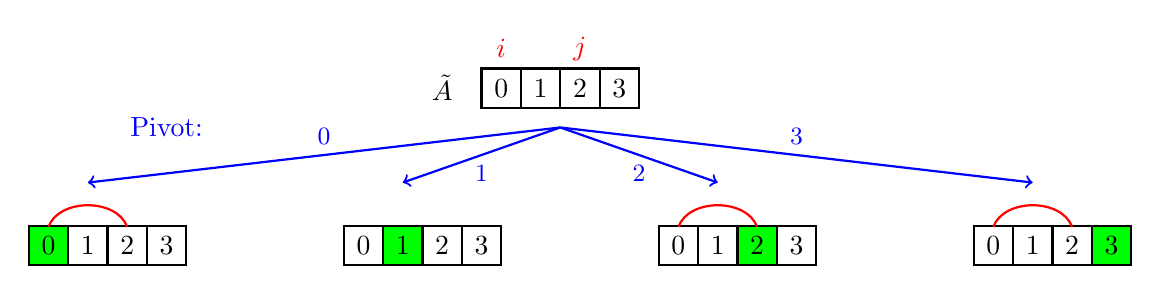
\begin{tikzpicture}[scale=1, auto,swap]
 
 %level 1
 \def\dx{0}
 \def\dy{0};
 
   \node[ultra thick] at ( - 0.5 + \dx -0.25, 0.25 + \dy) {$\tilde{A}$};

 
  \foreach \i/\name in { 0/0,1/1, 2/2, 3/3} {
         \draw[  fill=white, thick ]  (\i*0.5 + \dx -0.25,0 + \dy) rectangle (\i*0.5+0.5 + \dx - 0.25, 0.5 + \dy);
         \node (U\name) at (\i*0.5+0.25+ \dx -0.25, 0.5/2 + \dy) {$\name$};
 }
 
 \foreach \i/\name in { 0/0} {
         \node[ultra thick, red] at (\i*0.5+0.25+ \dx -0.25, 0.5/2 + \dy + 0.5) {$i$};
 }

 \foreach \i/\name in { 2/2} {
         \node[ultra thick, red] at (\i*0.5+0.25+ \dx -0.25, 0.5/2 + \dy + 0.5) {$j$};
 }
 
  \node[ultra thick, blue] at (0.5+0.25 - 5, 0.5/2 - 1 + 0.5) {Pivot:};
 
 %arrow 
     \draw[->,  thick, blue] ( 1*0.5 + 0.25+ \dx, 0.5/2 + \dy - 0.5) -- node[left, above]{\small $0$} (1*0.5 + 0.25+ \dx - 6, 0.5/2 + \dy - 2 + 0.8); 

     \draw[->,  thick, blue] ( 1*0.5 + 0.25+ \dx, 0.5/2 + \dy - 0.5) -- node[left, below]{\small $1$} (1*0.5 + 0.25+ \dx - 2, 0.5/2 + \dy - 2 + 0.8); 

     \draw[->,  thick, blue] ( 1*0.5 + 0.25+ \dx, 0.5/2 + \dy - 0.5) -- node[right, below]{\small $2$} (1*0.5 + 0.25+ \dx + 2, 0.5/2 + \dy - 2 + 0.8); 

     \draw[->,  thick, blue] ( 1*0.5 + 0.25+ \dx, 0.5/2 + \dy - 0.5) -- node[right, above]{\small $3$} (1*0.5 + 0.25+ \dx + 6, 0.5/2 + \dy - 2 + 0.8); 


 
 %level 2 
 %1 
 \def\dx{-6}
 \def\dy{-2};
  \foreach \i/\name in { 0/0,1/1,2/2, 3/3} {
         \draw[  fill=white, thick ]  (\i*0.5 + \dx,0 + \dy) rectangle (\i*0.5+0.5 + \dx, 0.5 + \dy);
         \node (U\name) at (\i*0.5+0.25+ \dx, 0.5/2 + \dy) {$\name$};
 }

   \foreach \i/\name in { 0/0} {
         \draw[  fill=green, thick ]  (\i*0.5 + \dx,0 + \dy) rectangle (\i*0.5+0.5 + \dx, 0.5 + \dy);
         \node (U\name) at (\i*0.5+0.25 + \dx, 0.5/2 + \dy) {$\name$};
 }

  %arc
    \draw[red, thick] (U2.north) to [out=180-70,in=70] (U0.north);


 %2 
 \def\dx{-2}
 \def\dy{-2};
  \foreach \i/\name in { 0/0,1/1,2/2, 3/3} {
         \draw[  fill=white, thick ]  (\i*0.5 + \dx,0 + \dy) rectangle (\i*0.5+0.5 + \dx, 0.5 + \dy);
         \node (U\name) at (\i*0.5+0.25+ \dx, 0.5/2 + \dy) {$\name$};
 }

   \foreach \i/\name in { 1/1} {
         \draw[  fill=green, thick ]  (\i*0.5 + \dx,0 + \dy) rectangle (\i*0.5+0.5 + \dx, 0.5 + \dy);
         \node (U\name) at (\i*0.5+0.25 + \dx, 0.5/2 + \dy) {$\name$};
 }

  %arc
 %   \draw[red, thick] (U3.north) to [out=180-70,in=70] (U1.north);


 %3 
 \def\dx{+2}
 \def\dy{-2};
  \foreach \i/\name in { 0/0,1/1,2/2, 3/3} {
         \draw[  fill=white, thick ]  (\i*0.5 + \dx,0 + \dy) rectangle (\i*0.5+0.5 + \dx, 0.5 + \dy);
         \node (U\name) at (\i*0.5+0.25+ \dx, 0.5/2 + \dy) {$\name$};
 }

   \foreach \i/\name in { 2/2} {
         \draw[  fill=green, thick ]  (\i*0.5 + \dx,0 + \dy) rectangle (\i*0.5+0.5 + \dx, 0.5 + \dy);
         \node (U\name) at (\i*0.5+0.25 + \dx, 0.5/2 + \dy) {$\name$};
 }

  %arc
    \draw[red, thick] (U2.north) to [out=180-70,in=70] (U0.north);



 %4 
 \def\dx{+6}
 \def\dy{-2};
  \foreach \i/\name in { 0/0,1/1,2/2, 3/3} {
         \draw[  fill=white, thick ]  (\i*0.5 + \dx,0 + \dy) rectangle (\i*0.5+0.5 + \dx, 0.5 + \dy);
         \node (U\name) at (\i*0.5+0.25+ \dx, 0.5/2 + \dy) {$\name$};
 }

   \foreach \i/\name in { 3/3} {
         \draw[  fill=green, thick ]  (\i*0.5 + \dx,0 + \dy) rectangle (\i*0.5+0.5 + \dx, 0.5 + \dy);
         \node (U\name) at (\i*0.5+0.25 + \dx, 0.5/2 + \dy) {$\name$};
 }

  %arc
    \draw[red, thick] (U2.north) to [out=180-70,in=70] (U0.north);
%  \draw[red, thick] (U4.north) to [out=60,in=180-60] (U5.north);
%  \draw[red, thick] (U4.north) to [out=70,in=180-70] (U6.north);
%  \draw[red, thick] (U4.north) to [out=80,in=180-80] (U7.north);	
%  
%    \draw[red, thick] (U4.north) to [out=180-60,in=60] (U3.north);
%  \draw[red, thick] (U4.north) to [out=180-70,in=70] (U2.north);
%  \draw[red, thick] (U4.north) to [out=180-80,in=80] (U1.north);	
  



\end{tikzpicture}

\caption{\fangsong 对包含4个元素的数组$A$运行{\sc QuickSort}算法排序时,$\tilde{A}[0]$和$\tilde{A}[2]$发生比较有两种可能:$(i)$ 当$\tilde{A}[0]$或$\tilde{A}[2]$被选做中心元时,在本轮迭代即进行比较;$(ii)$ 当$\tilde{A}[3]$被选做中心元时,$\tilde{A}[0], \tilde{A}[1], \tilde{A}[2]$被归入小数组$S_{-}$,并对$S_{-}$执行下一轮迭代;在下一轮迭代时可能发生比较,发生概率是$\frac{2}{3}$。}
\label{compareij4elements}
\end{figure}

\end{enumerate}

上述观察完全可以推广至数组包含$n$个元素的一般情况,即:
\begin{eqnarray}	
 \Pr( \tilde{A}[i]  \text{ is compared with } \tilde{A}[j] )  &=&  \frac{1}{n} + \frac{1}{n} +  \frac{n-(j-i+1)}{n} \times  \frac{2}{j-i+1}  \nonumber\\ 
 &=&  (\frac{j-i+1}{n} +  \frac{n-(j-i+1)}{n}) \times  \frac{2}{j-i+1}   \nonumber\\
 &=&  \frac{2}{j-i+1}\nonumber
 \end{eqnarray}

从而证明了两个元素$\tilde{A}[i]$和$\tilde{A}[j]$发生比较的概率是$\frac{2}{j-i+1}$,仅与元素的下标有关,和数组的大小$n$无关。

\subsubsection*{降低{\sc QuickSort}算法空间复杂度的努力:“原位”排序算法}
	上一小节所述的{\sc QuickSort}算法的时间复杂度很小,但是需要创建两个辅助数组$S_{-}$和$S_{+}$,这样一来,除了数组本身之外还要额外占用$n$个内存单元,导致当$n$比较大时,内存需求有时难以满足。因此,无需开辟额外的辅助空间、仅使用数组$A$所占的空间进行“原位”(In-place)排序,是很有实际价值的工作。
	
	xxx Lomuto和C. A. R. Hoare各自提出了一种“原位”{\sc QuickSort}算法;我们在此仅描述Lomuto的方法\cite{LomutoInPlaceQuickSort},Hoare的方法请见文献\cite{HoareInPlaceQuickSort}。
	
	{\bf 基本思想:} 为避免开辟辅助数组$S_{-}$和$S_{+}$,{\sc Lomuto}算法直接将数组$A$的左半部分当做$S_{-}$,存放比中心元小的元素;把数组$A$的右半部分当做$S_{+}$,存放比中心元大的元素(见图\ref{LomutoPartitionResults})。
	
	{\bf 算法设计与描述:} 数组分解这一步,{\sc Lomuto}算法是通过函数{\sc Partition}来完成的,其关键操作是“\uwave{交换}”,即:以$A[r]$作为中心元,比中心元小的元素放在$A[l..i-1]$区域,比中心元大的元素放在$A[i..j-1]$区域;下标$j$从$l$到$r$,逐个检验元素$A[j]$,若$A[j]$比中心元小,则交换$A[j]$和$A[i]$。最后将中心元放入正确的位置。
	
		Lomuto算法的伪代码描述如下:
	
\begin{algorithm}[H]
\caption{{\sc LomutoQuickSort} algorithm}\label{LomutoQuickSortAlgo} 
{\bf function} {\sc LomutoQuickSort}$(A, l, r)$ 
\begin{algorithmic}[1]
\IF{$l < r$} 
	\STATE{$p=${\sc Partition}$(A, l, r)$ //Use $A[r]$ as pivot}; 
	\STATE{{\sc LomutoQuickSort}$(A, l, \textcolor{red}{p-1})$}; 
	\STATE{{\sc LomutoQuickSort}$(A, p+1, r)$};
\ENDIF
\end{algorithmic}
\end{algorithm}

\begin{algorithm}[H]
\caption{{\sc Partition} algorithm used by {\sc LomutoQuickSort} }\label{LomutoPartitionAlgo} 
{\bf function} {\sc Partition}$(A, l, r)$ 
\begin{algorithmic}[1]
\STATE{$pivot=A[r]$;  $i=l$;}
\FOR{$j=l$ to $r-1$}
	\IF{$A[j] < pivot$}
		\STATE{Swap $A[i]$ with $A[j]$;}
		\STATE{$i++$;}
	\ENDIF
\ENDFOR
\STATE{Swap $A[i]$ with $A[r]$;} //Put pivot in its correct position
\RETURN{$i$};
\end{algorithmic}
\end{algorithm}


\begin{figure}[H]\centering
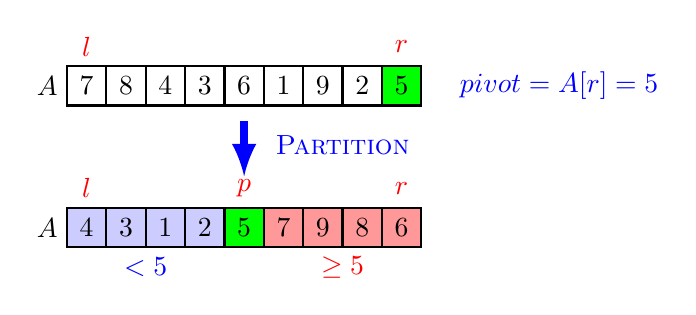
\begin{tikzpicture}[scale=1, auto,swap]
 
 %level 1
 \def\dx{0}
 \def\dy{0};
  \foreach \i/\name in { 0/7,1/8, 2/4, 3/3, 4/6, 5/1, 6/9, 7/2, 8/5} {
         \draw[  thick ]  (\i*0.5 + \dx,0 + \dy) rectangle (\i*0.5+0.5 + \dx, 0.5 + \dy);
         \node  at (\i*0.5+0.25+ \dx, 0.5/2 + \dy) {$\name$};
 }

  \foreach \i/\name in { 8/5} {
         \draw[  fill=green, thick ]  (\i*0.5 + \dx,0 + \dy) rectangle (\i*0.5+0.5 + \dx, 0.5 + \dy);
         \node  at (\i*0.5+0.25+ \dx, 0.5/2 + \dy) {$\name$};
 }

  \def\dy{0}; 
  \foreach \i/\name in { 12/pivot=A[r]=5} {
         \node [blue, ultra thick]  at (\i*0.5+0.25+ \dx, 0.5/2 + \dy) {$\name$};
 }
 
   \foreach \i/\name in { -1/A} {
         \node [ ultra thick]  at (\i*0.5+0.25+ \dx, 0.5/2 + \dy) {$\name$};
 }


 \def\dy{0.5}; 
   \foreach \i/\name in {  0/l, 8/r} {
          \node[red]  at (\i*0.5+0.25+ \dx, 0.5/2 + \dy) {$\name$};
 }
 
 
 %arrow
  \def\dx{0}
 \def\dy{0};
 \draw[blue, -latex, line width=3pt] (5*0.5-0.25 + \dx , -0.2 + \dy) -- (5*0.5-0.25+ \dx, -0.9+ \dy);

   \foreach \i/\name in { 6.5/Partition} {
         \node [blue, ultra thick]  at (\i*0.5+0.25+ \dx, 0.5/2 - 0.75 + \dy) {{\sc \name}};
 }


 %level 1
 \def\dx{0}
 \def\dy{-1.8};
  \foreach \i/\name in { 0/4,1/3, 2/1, 3/2 } {
         \draw[  fill=blue!20, thick ]  (\i*0.5 + \dx,0 + \dy) rectangle (\i*0.5+0.5 + \dx, 0.5 + \dy);
         \node  at (\i*0.5+0.25+ \dx, 0.5/2 + \dy) {$\name$};
 }
  \foreach \i/\name in {  5/7, 6/9, 7/8, 8/6} {
         \draw[  fill=red!40, thick ]  (\i*0.5 + \dx,0 + \dy) rectangle (\i*0.5+0.5 + \dx, 0.5 + \dy);
         \node  at (\i*0.5+0.25+ \dx, 0.5/2 + \dy) {$\name$};
 }


  \foreach \i/\name in { 4/5} {
         \draw[  fill=green, thick ]  (\i*0.5 + \dx,0 + \dy) rectangle (\i*0.5+0.5 + \dx, 0.5 + \dy);
         \node  at (\i*0.5+0.25+ \dx, 0.5/2 + \dy) {$\name$};
 }

 
   \foreach \i/\name in { -1/A} {
         \node [ ultra thick]  at (\i*0.5+0.25+ \dx, 0.5/2 + \dy) {$\name$};
 }


 \def\dy{0.5-1.8}; 
   \foreach \i/\name in {  0/l, 8/r, 4/p} {
          \node[red]  at (\i*0.5+0.25+ \dx, 0.5/2 + \dy) {$\name$};
 }
 
  \def\dy{0.5-2.8}; 
   \foreach \i/\name in {  1.5/} {
          \node[blue]  at (\i*0.5+0.25+ \dx, 0.5/2 + \dy) {$<5$};
 }
   \foreach \i/\name in {  6.5/} {
          \node[red]  at (\i*0.5+0.25+ \dx, 0.5/2 + \dy) {$\geq5$};
 } 
 
\end{tikzpicture}
\caption{\fangsong {\sc Lomuto}快速排序算法中使用的{\sc Partition}函数运行结果示例。}
\label{LomutoPartitionResults}
\end{figure}



\begin{figure}[H]\centering
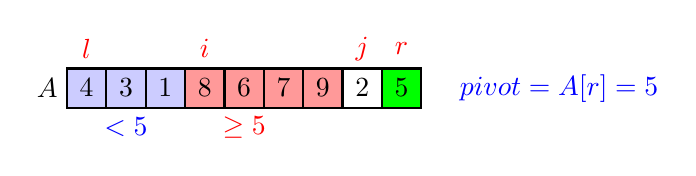
\begin{tikzpicture}[scale=1, auto,swap]
 
 %level 1
 \def\dx{0}
 \def\dy{0};
  \foreach \i/\name in { 0/4,1/3, 2/1, 3/8, 4/6, 5/7, 6/9, 7/2, 8/5} {
         \draw[  thick ]  (\i*0.5 + \dx,0 + \dy) rectangle (\i*0.5+0.5 + \dx, 0.5 + \dy);
         \node  at (\i*0.5+0.25+ \dx, 0.5/2 + \dy) {$\name$};
 }

  \foreach \i/\name in { 8/5} {
         \draw[  fill=green, thick ]  (\i*0.5 + \dx,0 + \dy) rectangle (\i*0.5+0.5 + \dx, 0.5 + \dy);
         \node  at (\i*0.5+0.25+ \dx, 0.5/2 + \dy) {$\name$};
 }

  \foreach \i/\name in { 0/4,1/3, 2/1} {
         \draw[  fill=blue!20, thick ]  (\i*0.5 + \dx,0 + \dy) rectangle (\i*0.5+0.5 + \dx, 0.5 + \dy);
         \node  at (\i*0.5+0.25+ \dx, 0.5/2 + \dy) {$\name$};
 }
 
  \foreach \i/\name in { 3/8, 4/6, 5/7, 6/9} {
         \draw[  fill=red!40, thick ]  (\i*0.5 + \dx,0 + \dy) rectangle (\i*0.5+0.5 + \dx, 0.5 + \dy);
         \node  at (\i*0.5+0.25+ \dx, 0.5/2 + \dy) {$\name$};
 }

  \def\dy{0}; 
  \foreach \i/\name in { 12/pivot=A[r]=5} {
         \node [blue, ultra thick]  at (\i*0.5+0.25+ \dx, 0.5/2 + \dy) {$\name$};
 }
 
   \foreach \i/\name in { -1/A} {
         \node [ ultra thick]  at (\i*0.5+0.25+ \dx, 0.5/2 + \dy) {$\name$};
 }


 \def\dy{0.5}; 
   \foreach \i/\name in {  0/l, 3/i, 7/j, 8/r} {
          \node[red]  at (\i*0.5+0.25+ \dx, 0.5/2 + \dy) {$\name$};
 }
 
 
 \def\dy{-0.5}; 
   \foreach \i/\name in {  1/} {
          \node[blue, ultra thick]  at (\i*0.5+0.25+ \dx, 0.5/2 + \dy) {$<5$};
 }
   \foreach \i/\name in {  4/} {
          \node[red, ultra thick]  at (\i*0.5+0.25+ \dx, 0.5/2 + \dy) {$\geq5$};
 } 
 
\end{tikzpicture}
\caption{\fangsong {\sc Lomuto}快速排序算法中使用的{\sc Partition}函数运行过程示例:当发现$A[j]$比中心元小时,则交换$A[j]$与$A[i]$。注意:$i$记录当前比中心元大的元素所在区域的最小下标。}
\label{LomutoPartition}
\end{figure}



%
%{\sc QuickSort}$(A, l, r)$ 
%\begin{algorithmic}[1]
%\IF{$l < r$} 
%	\STATE{$p=${\sc Partition}$(A, l, r)$ //Use $A[l]$ as pivot};
%	\STATE{{\sc QuickSort}$(A, l,  \textcolor{red}{p})$; \textcolor{red}{//Reason: $A[p]$ might not be at its correct position}}
%	\STATE{{\sc QuickSort}$(A, p+1, r)$};
%\ENDIF
%\end{algorithmic}
%
%
%\begin{itemize}
%	\item Sort the entire array: {\sc QuickSort}$(A, 0, n-1)$.
%\end{itemize}
%
%\begin{figure}[H]\centering
%\begin{tikzpicture}[scale=1, auto,swap]
% 
% %level 1
% \def\dx{0}
% \def\dy{0};
%  \foreach \i/\name in { 0/7,1/8, 2/4, 3/3, 4/6, 5/1, 6/9, 7/2, 8/5} {
%         \draw[  thick ]  (\i*0.5 + \dx,0 + \dy) rectangle (\i*0.5+0.5 + \dx, 0.5 + \dy);
%         \node  at (\i*0.5+0.25+ \dx, 0.5/2 + \dy) {$\name$};
% }
%
%  \foreach \i/\name in { 0/7} {
%         \draw[  fill=green, thick ]  (\i*0.5 + \dx,0 + \dy) rectangle (\i*0.5+0.5 + \dx, 0.5 + \dy);
%         \node  at (\i*0.5+0.25+ \dx, 0.5/2 + \dy) {$\name$};
% }
%
%  \def\dy{0}; 
%  \foreach \i/\name in { 12/pivot=A[l]=7} {
%         \node [blue, ultra thick]  at (\i*0.5+0.25+ \dx, 0.5/2 + \dy) {$\name$};
% }
% 
%   \foreach \i/\name in { -1/A} {
%         \node [ ultra thick]  at (\i*0.5+0.25+ \dx, 0.5/2 + \dy) {$\name$};
% }
%
%
% \def\dy{0.5}; 
%   \foreach \i/\name in {  0/l, 8/r} {
%          \node[red]  at (\i*0.5+0.25+ \dx, 0.5/2 + \dy) {$\name$};
% }
% 
% 
% %arrow
%  \def\dx{0}
% \def\dy{0};
% \draw[blue, -latex, line width=3pt] (5*0.5-0.25 + \dx , -0.2 + \dy) -- (5*0.5-0.25+ \dx, -0.9+ \dy);
%
%   \foreach \i/\name in { 6.5/Partition} {
%         \node [blue, ultra thick]  at (\i*0.5+0.25+ \dx, 0.5/2 - 0.75 + \dy) {{\sc \name}};
% }
%
%
% %level 2
% \def\dx{0}
% \def\dy{-1.8};
%  \foreach \i/\name in { 0/5,1/2, 2/4, 3/3, 4/6, 5/1   } {
%         \draw[  fill=blue!20, thick ]  (\i*0.5 + \dx,0 + \dy) rectangle (\i*0.5+0.5 + \dx, 0.5 + \dy);
%         \node  at (\i*0.5+0.25+ \dx, 0.5/2 + \dy) {$\name$};
% }
%  \foreach \i/\name in {  6/9, 7/8, 8/7} {
%         \draw[  fill=red!40, thick ]  (\i*0.5 + \dx,0 + \dy) rectangle (\i*0.5+0.5 + \dx, 0.5 + \dy);
%         \node  at (\i*0.5+0.25+ \dx, 0.5/2 + \dy) {$\name$};
% }
%
% 
%   \foreach \i/\name in { -1/A} {
%         \node [ ultra thick]  at (\i*0.5+0.25+ \dx, 0.5/2 + \dy) {$\name$};
% }
%
%
% \def\dy{0.5-1.8}; 
%   \foreach \i/\name in {  0/l, 8/r, 5/p} {
%          \node[red]  at (\i*0.5+0.25+ \dx, 0.5/2 + \dy) {$\name$};
% }
% 
%  \def\dy{0.5-2.8}; 
%   \foreach \i/\name in {  1.5/} {
%          \node[blue]  at (\i*0.5+0.25+ \dx, 0.5/2 + \dy) {$\leq7$};
% }
%   \foreach \i/\name in {  6.5/} {
%          \node[red]  at (\i*0.5+0.25+ \dx, 0.5/2 + \dy) {$\geq7$};
% } 
% 
%\end{tikzpicture}
%\end{figure}
%
%
%
%\begin{figure}[H]\centering
%\begin{tikzpicture}[scale=1, auto,swap]
% 
% %level 1
% \def\dx{0}
% \def\dy{0};
%  \foreach \i/\name in { 0/5,1/2, 2/4, 3/3, 4/6, 5/1, 6/9, 7/8, 8/7} {
%         \draw[  thick ]  (\i*0.5 + \dx,0 + \dy) rectangle (\i*0.5+0.5 + \dx, 0.5 + \dy);
%         \node  at (\i*0.5+0.25+ \dx, 0.5/2 + \dy) {$\name$};
% }
%
%
%
%  \foreach \i/\name in { 0/5,1/2, 2/4, 3/3} {
%         \draw[  fill=blue!20, thick ]  (\i*0.5 + \dx,0 + \dy) rectangle (\i*0.5+0.5 + \dx, 0.5 + \dy);
%         \node  at (\i*0.5+0.25+ \dx, 0.5/2 + \dy) {$\name$};
% }
%  \foreach \i/\name in { 6/9, 7/8, 8/7} {
%         \draw[  fill=red!40, thick ]  (\i*0.5 + \dx,0 + \dy) rectangle (\i*0.5+0.5 + \dx, 0.5 + \dy);
%         \node  at (\i*0.5+0.25+ \dx, 0.5/2 + \dy) {$\name$};
% }
%
%  \def\dy{0}; 
%  \foreach \i/\name in { 12/pivot=A[l]=7} {
%         \node [blue, ultra thick]  at (\i*0.5+0.25+ \dx, 0.5/2 + \dy) {$\name$};
% }
% 
%   \foreach \i/\name in { -1/A} {
%         \node [ ultra thick]  at (\i*0.5+0.25+ \dx, 0.5/2 + \dy) {$\name$};
% }
%
%
% \def\dy{0.5}; 
%   \foreach \i/\name in {  0/l, 4/i, 5/j, 8/r} {
%          \node[red]  at (\i*0.5+0.25+ \dx, 0.5/2 + \dy) {$\name$};
% }
% 
% 
% \def\dy{-0.5}; 
%   \foreach \i/\name in {  1.5/} {
%          \node[blue, ultra thick]  at (\i*0.5+0.25+ \dx, 0.5/2 + \dy) {$\leq7$};
% }
%   \foreach \i/\name in {  7/} {
%          \node[red, ultra thick]  at (\i*0.5+0.25+ \dx, 0.5/2 + \dy) {$\geq7$};
% } 
% 
%\end{tikzpicture}
%\end{figure}
%
%
%
%\begin{algorithm}[H]
%\caption{{\sc InsertionSort} algorithm}\label{InsertionSortAlgo} 
%{\bf function} {\sc Partition}$(A, l, r)$ 
%\begin{algorithmic}[1]
%\STATE{$i=l-1$; $j=r+1$; $pivot=A[l]$;}
%\WHILE{{\tt TRUE}}
%	\REPEAT
%		\STATE{$j=j-1$; //From right to left, find the first element $\leq pivot$} 
%	\UNTIL{$A[j]\leq pivot$ or $j == l$ }; 
%	\REPEAT
%		\STATE{$i=i+1$;  //From left to right, find the first element $\geq pivot$} 
%	\UNTIL{$A[i]\geq pivot$ or $i == r$}; 
%	\IF{$j\leq i$}
%		\RETURN $j$;
%	\ENDIF
%	\STATE{Swap $A[i]$ with $A[j]$;}
%\ENDWHILE
%\end{algorithmic}
%\end{algorithm}
%
%\begin{itemize}
%	\item Sort the entire array: {\sc QuickSort}$(A, 0, n-1)$.
%\end{itemize}


\subsubsection*{算法性能比较}
    Hoare做了一个有趣的实验,比较了{\sc MergeSort}和{\sc QuickSort}的性能。如表\ref{HoareComparisonTable}所示,对越大的数组,{\sc QuickSort}算法的性能优势越显著。由于Hoare使用的405型计算机内存大小有限,表格中的带``*''的数据是Hoare使用公式推算出来的。
     \begin{table}[h!]
     \centering
    {\begin{tabular}{rrr}
    \hline
                                                &  \multicolumn{2}{c}{\fangsong 运行时间}  \\
                         \cline{2-3}
             {\fangsong 数组大小$n$}  & {\sc MergeSort} {\fangsong 算法}   & {\sc QuickSort} {\fangsong 算法} \\
      \hline          
      		500 & 2 min 8 sec & 1 min 21 sec \\ 
 		1000 & 4 min 48 sec & 3 min 8 sec \\  
                  1500 & 8 min 15 sec* & 5 min 6 sec \\
                  2000 & 11 min 0 sec * & 6 min 47 sec \\
       \hline          
    \end{tabular}}{}
    \caption{\fangsong {\sc MergeSort}算法和{\sc QuickSort}算法性能比较\cite{Hoare1961}。}
 	\label{HoareComparisonTable}
    \end{table}
    
    还应该说明的是:迄今为止我们都是假设数组中的元素各不相同;当数组中存在重复元素时,上述{\sc QuickSort}算法性能不好。为克服这种缺陷,一种简单的改进方式是在分解数组时,不是简单地分成两个小数组$S_{-}$和$S_{+}$,而是分成三个小数组:比中心元小的放入$S_{-}$,比中心元大的放入$S_{+}$,以及和中心元相等的元素。
    


\section{一个密切相关的问题:数组中的逆序对计数}

和数组排序密切相关的一个问题是:如何对数组中的“逆序对”进行计数。所谓逆序对,是指数组中的两个元素$A[i]$和$A[j]$,其下标$i < j$,但是考察元素的值,却有$A[i] > A[j]$。比如数组$A=[2, 4, 1, 3, 5]$中,共存在3个逆序对,即$2$和$1$、$4$和$1$、$4$和$3$。逆序对计数问题可形式化描述如下:

\begin{center}
 	\fbox{
 		\begin{minipage}{33em}
 {\bf 逆序对计数问题(Inversion-counting problem)}\\
 	{\bf 输入:} 一个包含$n$个元素的数组$A[0..n-1]$;\\
 	{\bf 输出:} 数组中的逆序对的数目。
 		\end{minipage}
 	}
\end{center}


 数组的逆序对计数是一项基本运算,有着广泛的应用。例如在衡量两个变量的相关程度时,可以使用Spearman系数$\rho$和Kendall系数$\tau$来衡量“秩”相关程度(Rank correlation),其中 Kendall系数$\tau$可以归结为逆序数的计算\cite{Kendall1938}。

给定一个数组,我们可以依据逆序对的定义,用两重{\tt for}循环即可计算出逆序对的数目。不过这种直接依据定义的算法的时间复杂度是$O(n^2)$,那么能否设计出更高效的算法呢?

我们依然从最简单的实例入手:如果数组$A$只有两个元素$A[0]$和$A[1]$,我们只需比较这两个元素,即可计算出逆序数。

下面考虑如何求解规模更大的实例。考虑包含$n$个元素的数组$A$,我们可以很容易地依据下标将$A$分解成两个小的数组,
即左一半$A[0..\lceil\frac{n}{2}\rceil-1]$和右一半$A[\lceil\frac{n}{2}\rceil..n-1]$。
在将大的实例分解成子实例之后,我们可以假定子实例已经求解,即使用递归调用分别求出两个元素都在左一半中的逆序对数目、以及两个元素都在右一半中的逆序对数目。
现在只剩下最后一个困难:如何将子实例的解“组合”成原始给定实例的解;这需要对一个元素在左一半、另一个元素在右一半所构成的逆序对进行计数。

一种直接的“组合”方法如图\ref{InversionCountingSimpleMerge}所示:检查所有的一个在左一半、一个在右一半的元素对,对其中出现的逆序对进行计数。可是这种“组合”方法的时间复杂度是$O(n^2)$,从而导致整个算法的时间复杂度是:
\[
	T(n) = 2T(\tfrac{n}{2}) + O(n^2) = O(n^2) 
\]


%\begin{figure}[H]\centering
% 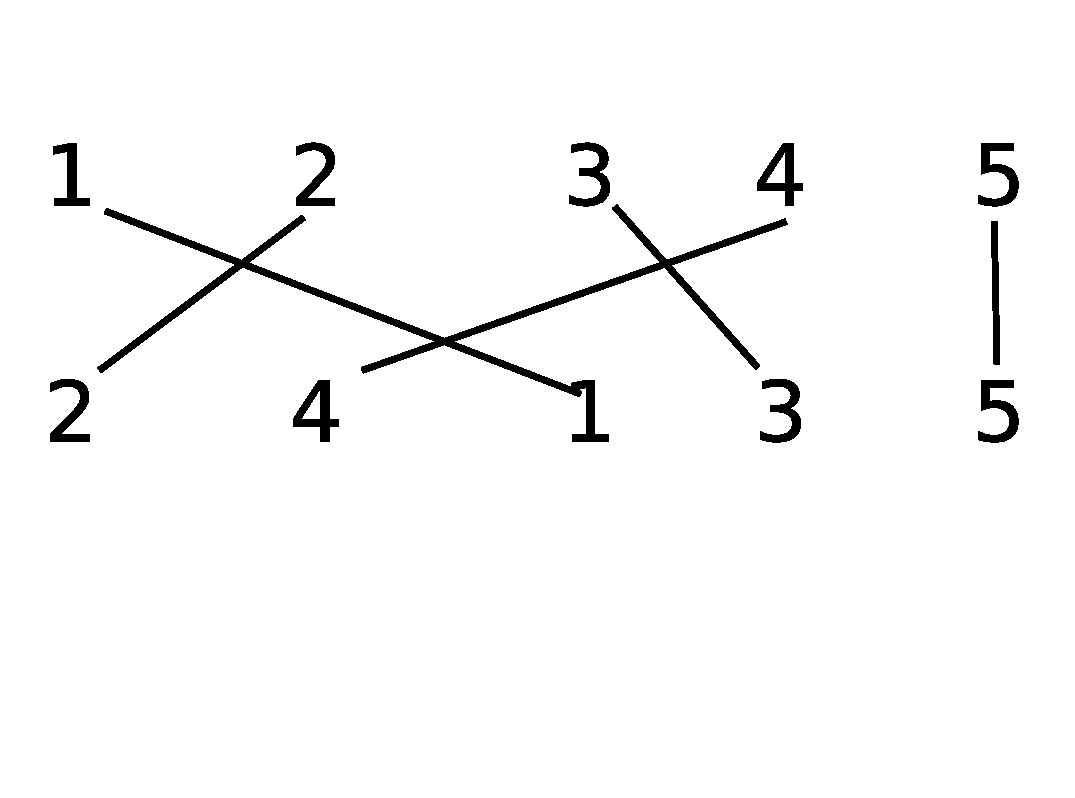
\includegraphics[width=2in] {L5-counting-inversion.eps}
%\end{figure}
%

%
%\begin{figure}[H]\centering
%    
%\begin{tikzpicture}[scale=1., auto,swap]
% 
%  \foreach \i/\name in { 0/5,1/2,2/3,3/1,4/7, 5/8, 6/6, 7/4 } {
%         \draw[  fill=white, thick ] (\i*0.5,0) rectangle (\i*0.5+0.5, 0.5);
%         \node at (\i*0.5+0.25, 0.5/2) {$\name$};
% }
% 
%
% %level 2
%  
%   \foreach \i/\name\n in { 0/5/s2,1/2/s5,2/3/s5,3/1/s1 } {
%         \draw[  fill=white, thick ] (\i*0.5-1,0-1) rectangle (\i*0.5-1+0.5, 0.5-1);
%         \node (\n) at (\i*0.5+0.25-1, 0.5/2-1) {$\name$};
% }
% 
%    \foreach \i/\name/\n in { 4/7/s7, 5/8/s4, 6/6/s6, 7/4/s8 } {
%         \draw[  fill=white, thick ] (\i*0.5+1,0-1) rectangle (\i*0.5+1+0.5, 0.5-1);
%         \node (\n) at (\i*0.5+0.25+1, 0.5/2-1) {$\name$};
% }
% 
%  
% % lines 
% \foreach \source/\dest in {{( 4*0.5 , 0)/( 2*0.5 - 1, -0.5)}, {( 4*0.5 , 0)/( 6*0.5 + 1, -0.5)}} 
% 	\path[draw=red, ->, thick]  \source  --  \dest;
% 
%	
%  
%%\end{tikzpicture}
%%\caption{\fangsong }
%%\label{InversionCountingSimpleMerge}
%%\end{figure}
%%
%%
\begin{figure}[H]\centering
    
\begin{tikzpicture}[scale=1., auto,swap]
 
\def\dx{-7};
 
  \foreach \i/\name in { 0/5,1/2,2/3,3/1,4/7, 5/8, 6/6, 7/4 } {
         \draw[  fill=white, thick ] (\i*0.5 + \dx,0) rectangle (\i*0.5+0.5 + \dx, 0.5);
         \node at (\i*0.5+0.25 + \dx, 0.5/2) {$\name$};
 }

 %level 2
  
   \foreach \i/\name/\n in { 0/5/s2,1/2/s5,2/3/s3,3/1/s1} {
         \draw[  fill=white, thick ] (\i*0.5-1 + \dx,0-1) rectangle (\i*0.5-1+0.5 + \dx, 0.5-1);
         \node (\n) at (\i*0.5+0.25-1 + \dx, 0.5/2-1) {$\name$};
 }
 
    \foreach \i/\name/\n in { 4/7/s7, 5/8/s4, 6/6/s6, 7/4/s8} {
         \draw[  fill=white, thick ] (\i*0.5+1 + \dx,0-1) rectangle (\i*0.5+1+0.5 + \dx, 0.5-1);
         \node (\n) at (\i*0.5+0.25+1 + \dx, 0.5/2-1) {$\name$};
 }
 
  
 % lines 
 \foreach \source/\dest in {{( 4*0.5  + \dx, 0)/( 2*0.5 - 1 + \dx, -0.5)}, {( 4*0.5  + \dx, 0)/( 6*0.5 + 1 + \dx, -0.5)}} 
 	\path[draw=red, ->, thick]  \source  --  \dest;
 
\draw[green, dashed, thick] (s1.south) to [out=-30, in=180+30] (s7.south);
\draw[green, dashed, thick] (s1.south) to [out=-35, in=180+35] (s4.south);
\draw[green, dashed, thick] (s1.south) to [out=-40, in=180+40] (s6.south);
\draw[green, dashed, thick] (s1.south) to [out=-45, in=180+45] (s8.south);

\draw[green, dashed, thick] (s3.south) to [out=-35, in=180+35] (s7.south);
\draw[green, dashed, thick] (s3.south) to [out=-40, in=180+40] (s4.south);
\draw[green, dashed, thick] (s3.south) to [out=-45, in=180+45] (s6.south);
\draw[green, dashed, thick] (s3.south) to [out=-50, in=180+50] (s8.south);

\draw[green, dashed, thick] (s5.south) to [out=-40, in=180+40] (s7.south);
\draw[green, dashed, thick] (s5.south) to [out=-45, in=180+45] (s4.south);
\draw[green, dashed, thick] (s5.south) to [out=-50, in=180+50] (s6.south);
\draw[green, dashed, thick] (s5.south) to [out=-55, in=180+55] (s8.south);

\draw[green, dashed, thick] (s2.south) to [out=-45, in=180+45] (s7.south);
\draw[green, dashed, thick] (s2.south) to [out=-50, in=180+50] (s4.south);
\draw[green, dashed, thick] (s2.south) to [out=-55, in=180+55] (s6.south);
\draw[green, dashed, thick] (s2.south) to [out=-60, in=180+60] (s8.south);



%\end{tikzpicture}
%
%\end{figure}
%
%
%\begin{figure}[H]\centering
%    
%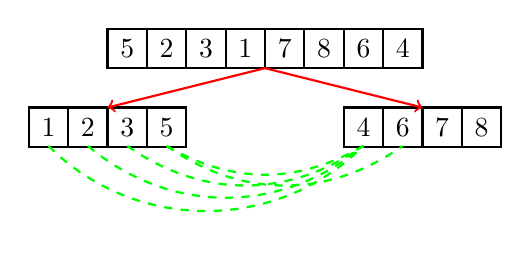
\begin{tikzpicture}[scale=1., auto,swap]
 
  \foreach \i/\name in { 0/5,1/2,2/3,3/1,4/7, 5/8, 6/6, 7/4 } {
         \draw[  fill=white, thick ] (\i*0.5,0) rectangle (\i*0.5+0.5, 0.5);
         \node at (\i*0.5+0.25, 0.5/2) {$\name$};
 }

 %level 2
  
   \foreach \i/\name/\n in { 0/1/s1,1/2/s2,2/3/s3,3/5/s5} {
         \draw[  fill=white, thick ] (\i*0.5-1,0-1) rectangle (\i*0.5-1+0.5, 0.5-1);
         \node (\n) at (\i*0.5+0.25-1, 0.5/2-1) {$\name$};
 }
 
    \foreach \i/\name/\n in { 4/4/s4, 5/6/s6, 6/7/s7, 7/8/s8} {
         \draw[  fill=white, thick ] (\i*0.5+1,0-1) rectangle (\i*0.5+1+0.5, 0.5-1);
         \node (\n) at (\i*0.5+0.25+1, 0.5/2-1) {$\name$};
 }
 
  
 % lines 
 \foreach \source/\dest in {{( 4*0.5 , 0)/( 2*0.5 - 1, -0.5)}, {( 4*0.5 , 0)/( 6*0.5 + 1, -0.5)}} 
 	\path[draw=red, ->, thick]  \source  --  \dest;
 
\draw[green, dashed, thick] (s5.south) to [out=-30, in=180+30] (s4.south);
\draw[green, dashed, thick] (s3.south) to [out=-35, in=180+35] (s4.south);
\draw[green, dashed, thick] (s2.south) to [out=-40, in=180+40] (s4.south);
\draw[green, dashed, thick] (s1.south) to [out=-45, in=180+45] (s4.south);

\draw[green, dashed, thick] (s5.south) to [out=-35, in=180+35] (s6.south);


\end{tikzpicture}
\caption{\fangsong 逆序对计数算法中“组合”子问题的解的两种策略:}
\label{InversionCountingMerge}
\end{figure}

那么能否更高效地进行“组合”呢?这里的一个关键性的思考是:如果左一半和右一半是任意的、没有任何结构的,我们没有别的办法,只能采用上述简单的逐对检查策略。



{\sc Sort-and-Count}$(A)$
\begin{algorithmic}[1]
\STATE Divide $A$ into two sub-sequences $L$ and $R$;
\STATE $(RC_L, L)$ = {\sc Sort-and-Count}$(L)$;
\STATE $(RC_R, R)$ = {\sc Sort-and-Count}$(R)$;
\STATE $(C, A)$ = {\sc Merge-and-Count}$(L,R)$;
\RETURN{$ (RC=RC_L+RC_R+C, A);$}
\end{algorithmic}
{\sc Merge-and-Count} $(L,R)$
\begin{algorithmic}[1]
\STATE $RC = 0;$ $ i=0; $ $j=0;$
\FOR{ $k=0$ to $\|L\|+\|R\|-1$ }
	\IF { $L[i] > R[j] $}
		\STATE $A[k] = R[j];$
		\STATE $j++;$
		\STATE \textcolor{red}{\bf $RC += (\|L\| - i);$}
	\ELSE 
		\STATE $A[k] = L[i];$
		\STATE $i++;$
	\ENDIF
\ENDFOR
\RETURN{($RC$, $A$); }
\end{algorithmic}
Time complexity: $T(n)=2T(\tfrac{n}{2}) + O(n) = O(n\log n)$. 


\section*{延伸阅读}


数组的逆序对计数是一项基本运算,有着广泛的应用。例如在衡量两个变量的相关程度时,通常可以使用Pearson相关系数衡量两个变量$x$和$y$的线性相关程度,或者使用Spearman系数$\rho$和Kendall系数$\tau$来衡量“秩”相关程度(Rank correlation);其中 Kendall系数$\tau$可以归结为逆序数的计算\cite{Kendall1938}。详细地说,考察变量$X$和$Y$的$n$次采样$x_1, x_2, ..., x_n$和$y_1, y_2, ..., y_n$,Kendall相关系数定义如下:
 \[
 	\tau = \frac{2}{n(n-1)} \sum_{i < j} sgn(x_i - x_j ) sgn(y_i - y_j)
 \]
H. Huang等对Kendal系数做了进一步的发展,提出了一种新的统计量,可以刻画变量的“局部秩相关性”\cite{Huang2014PNAS}。


	\begin{itemize}
	\item 
When the data changes gradually, the goal of a sorting algorithm is to sort the data at each time step, under the constraint that it only has limited access to the data each time.
\item As the data is constantly changing and the algorithm might be unaware of these changes, it cannot be expected to always output the exact right solution; we are interested in algorithms that guarantee to output an approximate solution.
\item In 2011, Eli Upfal et al. proposed an algorithm to sort dynamic data. 
\item In 2017, Liu and Huang proposed an efficient algorithm to determine top $k$ elements of dynamic data. 
\end{itemize} 


动态数据排序

曾刚
	
	
	
\section*{习题}	
\begin{enumerate}[1.]
	\item 比较如下的复杂度函数
\end{enumerate}	
		
